\chapter{内隐记忆的细胞机制和个性的生物基础} \label{chap:chap53}

在这本书中,我们一直强调所有行为都是大脑的一种功能,而大脑的功能障碍会产生特征性的行为障碍。
行为也受经验影响。
经验如何作用于大脑的神经回路以改变行为?
大脑如何获取新信息,一旦获取,又如何存储、检索和记忆?


在上一章中,我们看到记忆不是一个单一的过程,而是至少有两种主要形式。
内隐记忆是在无意识和自动的情况下运作的,例如在条件反射、习惯、知觉和运动技能的记忆中,而外显记忆是有意识地运作的,例如在对人、地点和物体的记忆中。
用于长期记忆存储的回路在显性和隐性记忆之间有所不同。
外显记忆的长期储存始于海马体和新皮层的内侧颞叶,而不同类型的内隐记忆的长期储存需要一系列神经结构:
负责启动的新皮层、负责技能和习惯的纹状体、 杏仁核用于巴甫洛夫威胁条件反射(也称为恐惧条件反射),小脑用于学习运动技能,以及用于非联想学习的某些反射通路,如习惯化和敏感化(图~\ref{fig:53_1})。


\begin{figure}[htbp]
	\centering
	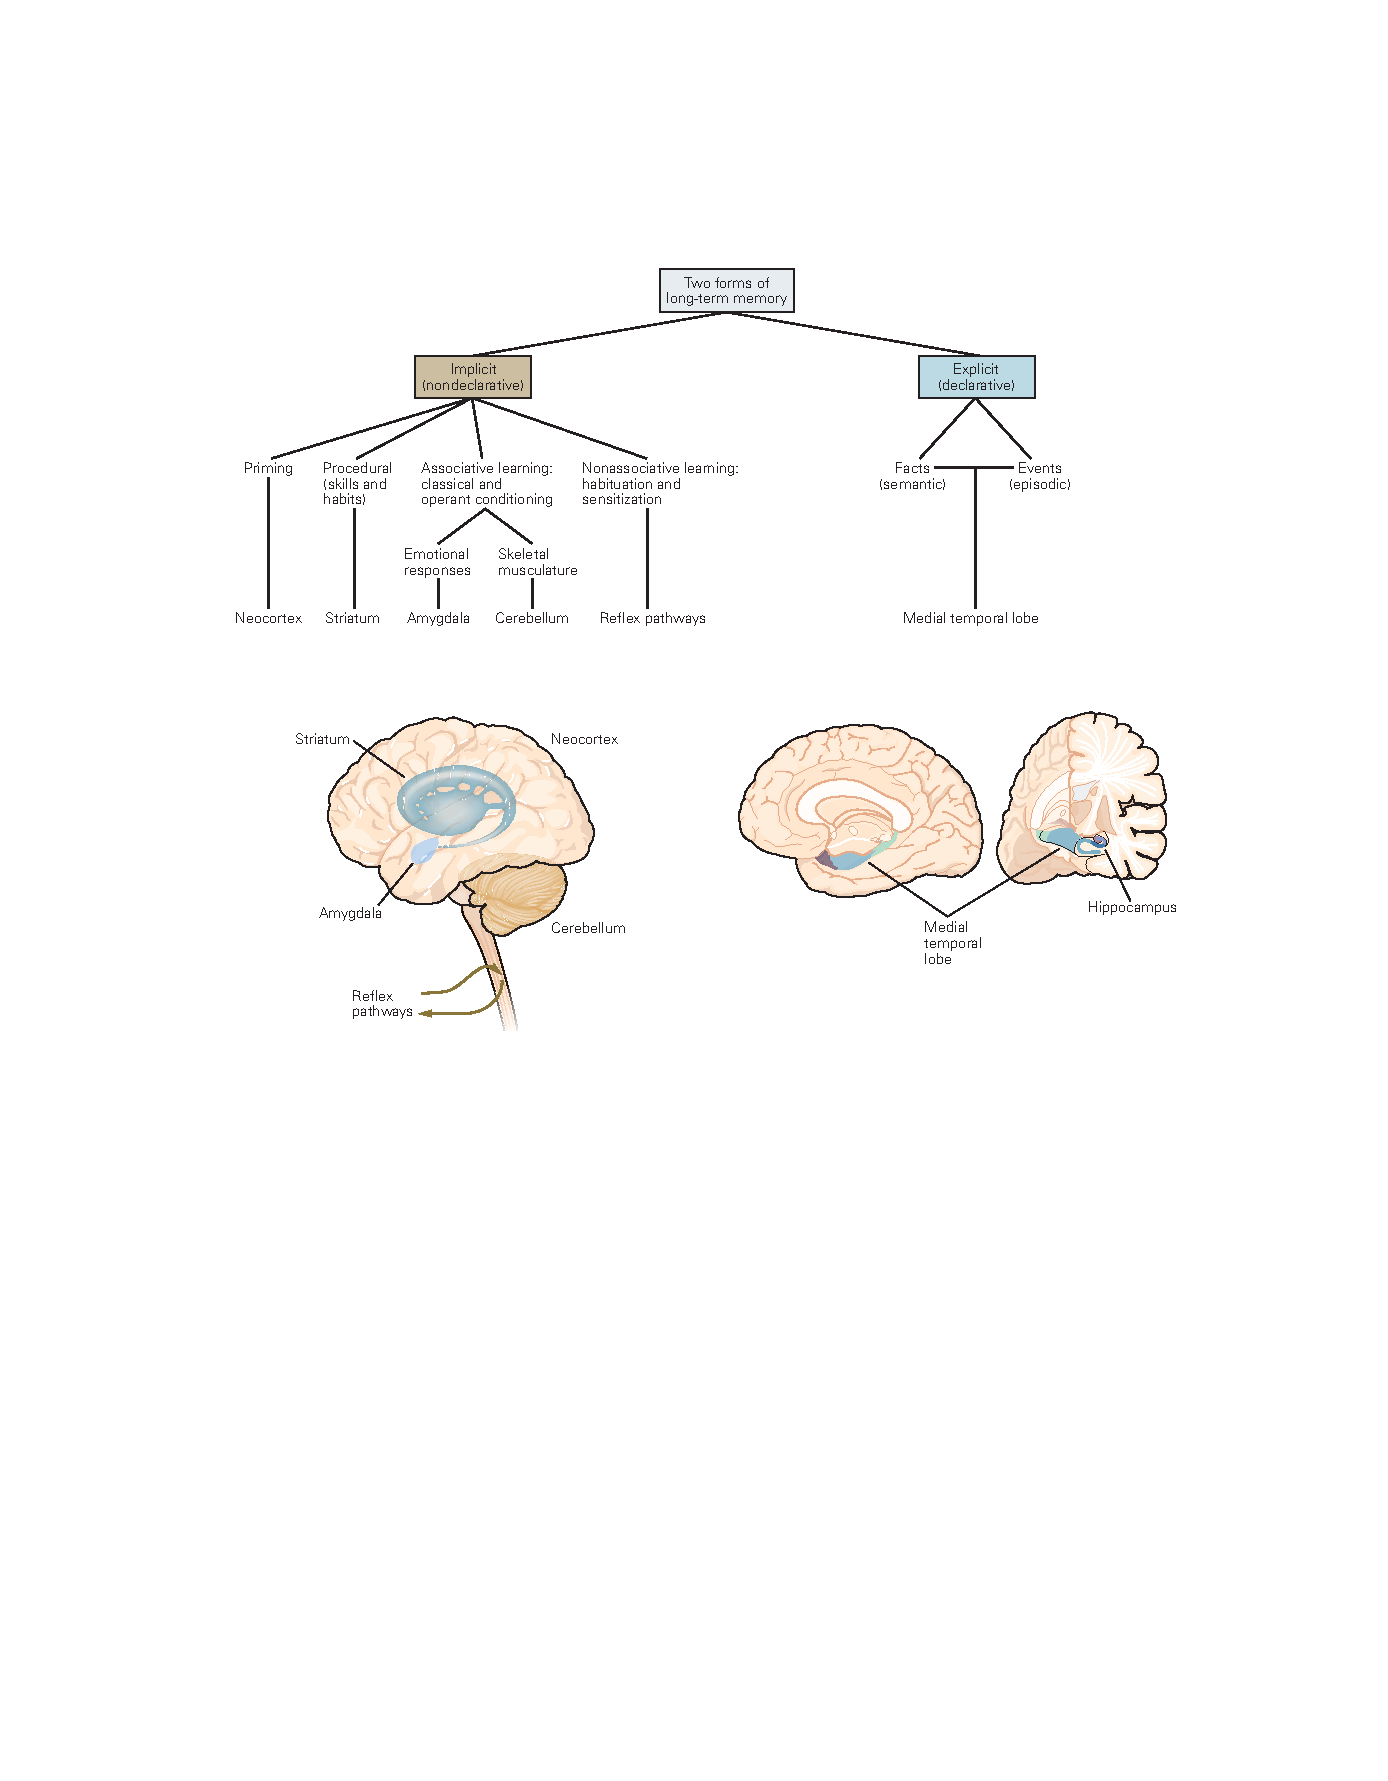
\includegraphics[width=0.9\linewidth]{chap53/fig_53_1}
	\caption{两种形式的长期记忆涉及不同的大脑系统。
		内隐记忆涉及新皮层、纹状体、杏仁核、小脑,在最简单的情况下,还涉及反射通路本身。
		外显记忆需要内侧颞叶和海马体,以及新皮层的某些区域(未显示)。}
	\label{fig:53_1}
\end{figure}


随着时间的推移,外显记忆被转移到新皮层的不同区域。
此外,我们最初存储为外显记忆的许多认知、运动和感知技能最终在实践中变得根深蒂固,以至于它们被存储为内隐记忆。
从外显记忆到内隐记忆的转移以及它们之间的差异在英国音乐家和指挥家\textit{克里夫·韦林}的案例中得到了戏剧性的证明,他在 1985 年遭受了大脑病毒感染(疱疹性脑炎),影响了海马体和颞叶皮层。
\textit{韦林}对他一两分钟前遇到的事件或人的记忆严重丧失,但他阅读音乐、弹钢琴或进行合唱的能力未受影响。
然而,一旦表演完成,他就什么都不记得了。


同样,抽象表现主义画家\textit{威廉·德·库宁}因阿尔茨海默病而出现严重的外显记忆障碍。
随着疾病的进展以及他对人物、地点和物体的记忆力下降,他仍然继续创作重要而有趣的画作。
他的创造性人格的这一方面相对未受影响。


在本章中,我们将研究构成无脊椎动物和脊椎动物内隐记忆存储基础的细胞和分子机制。
我们专注于了解威胁(有时称为恐惧学习)。
第~\ref{chap:chap37}~章和第~\ref{chap:chap38}~章讨论了涉及小脑和基底神经节的哺乳动物运动技能和习惯的内隐记忆。
在下一章中,我们将研究哺乳动物外显记忆的生物学。



\section{内隐记忆的存储涉及突触传递有效性的变化}

内隐学习的基本形式(习惯化、敏感化和经典条件反射)的研究为研究记忆存储的神经机制提供了概念框架。
这种学习已经在简单的无脊椎动物和各种脊椎动物行为中进行了分析,例如屈曲和眨眼反射,以及防御行为,例如冻结。
这些简单形式的内隐记忆涉及调节行为的突触通路有效性的变化。



\subsection{突触传递的突触前抑制导致习惯化}

习惯化是最简单的内隐学习形式。
例如,当动物学会忽略新刺激时,就会发生这种情况。
动物通过一系列定向反应对新刺激作出反应。
如果刺激既无益也无害,动物会在反复接触后学会忽略它。


\textit{查尔斯·谢林顿}在研究猫的姿势和运动时首先研究了这种行为的生理学基础。
\textit{谢林顿}观察到某些反射的强度会随着对运动通路的反复电刺激而减弱。
他认为这种他称之为习惯的减少是由受刺激通路中的突触有效性降低引起的。


习惯后来被\textit{奥尔登·斯宾塞}和\textit{理查德·汤普森}在细胞水平上进行了研究。
他们发现猫的脊柱屈曲反射习惯(从有害刺激中撤回肢体)与更复杂的人类行为习惯之间存在密切的细胞和行为相似之处。
他们表明,在习惯化过程中,从局部兴奋性中间神经元到脊髓运动神经元的输入强度下降,而从支配皮肤的感觉神经元到相同中间神经元的输入没有变化。


由于脊椎动物脊髓中间神经元的组织非常复杂,因此很难进一步分析屈曲反射中习惯化的细胞机制。
进步需要一个更简单的系统。
海洋软体动物\textit{海兔}拥有一个由大约 2 万个中枢神经元组成的简单神经系统,被证明是研究内隐记忆形式的绝佳系统。


海兔有一套防御反射系统,可以缩回它的呼吸鳃和虹吸管,鳃上方有一个小的肉质喷口,用于排出海水和废物(图~\ref{fig:53_2}A)。
这些反射类似于\textit{斯宾塞}和\textit{汤普森}研究的腿部退缩反射。
虹吸管的轻度触摸引起虹吸管和鳃的反射性缩回。
通过反复刺激,这些反射会形成习惯。
正如我们将要看到的,这些反应也可以是去习惯化的、敏感的和经典条件反射的。


\begin{figure}[htbp]
	\centering
	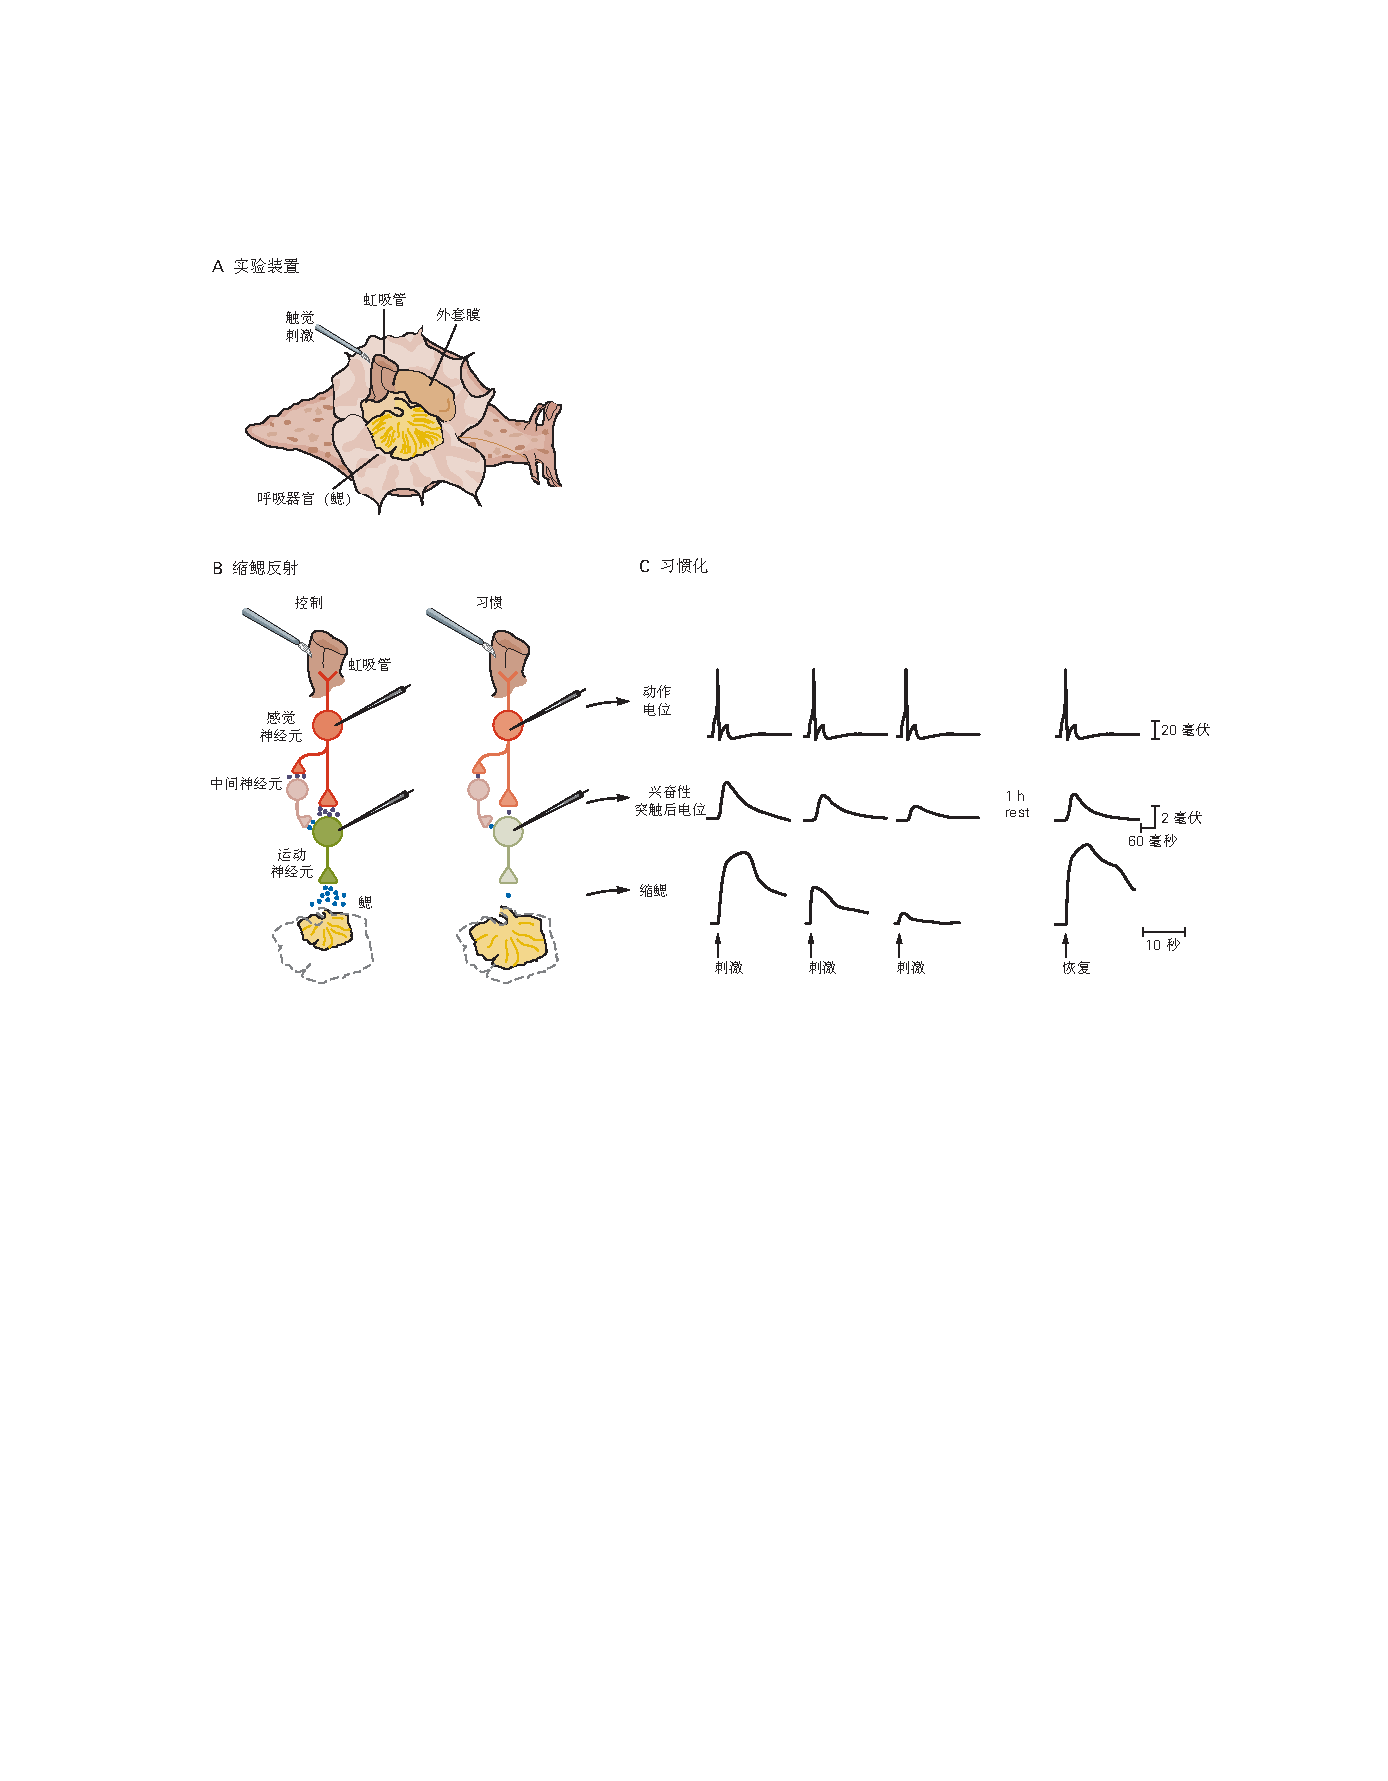
\includegraphics[width=1.0\linewidth]{chap53/fig_53_2}
	\caption{海蜗牛\textit{海兔}的\textit{缩鳃反射}的短期习惯。
		\textbf{A.} \textit{海兔}的背视图展示了呼吸器官(鳃)和\textit{外套膜},它以虹吸管结束,虹吸管是一种用于排出海水和废物的肉质喷口。
		触摸虹吸管会引起\textit{缩鳃反射}。
		反复刺激会导致习惯。
		\textbf{B.} \textit{缩鳃反射}回路和习惯化部位的简化图。
		腹部神经节中大约 24 个机械感受器神经元支配虹吸管皮肤。
		这些感觉细胞在支配鳃的六个运动神经元以及调节运动神经元放电的中间神经元上形成兴奋性突触。
		(为简单起见,此处仅说明了每种类型的神经元中的一个。)触摸虹吸管会导致鳃退缩(虚线轮廓显示原始鳃大小;实线轮廓显示最大退缩)。
		\textbf{C.} 反复刺激虹吸管感觉神经元(顶部痕迹)导致感觉神经元和运动神经元之间的突触传递逐渐抑制。
		尽管突触前\textit{动作电位}没有变化,但运动神经元\textit{兴奋性突触后电位}的大小逐渐减小。
		在一个单独的实验中,虹吸管的反复刺激导致鳃退缩(习惯化)的减少。
		重复刺激一小时后,\textit{兴奋性突触后电位}和退鳃都已恢复。
		习惯化涉及整个反射回路中许多突触位点的递质释放减少\cite{pinsker1970habituation}。}
	\label{fig:53_2}
\end{figure}


已经详细研究了调节海兔\textit{缩鳃反射}的神经回路。
触摸虹吸管会激发一组支配虹吸管的机械感受器感觉神经元。
感觉神经元末梢释放的谷氨酸在中间神经元和运动细胞中产生快速\textit{兴奋性突触后电位}。
来自感觉细胞和中间神经元的\textit{兴奋性突触后电位}在时间和空间上对运动细胞进行总结,导致它们强烈放电,从而使鳃有力地收缩。
然而,如果重复触摸虹吸管,中间神经元和运动细胞中的感觉神经元产生的单突触\textit{兴奋性突触后电位}会逐渐减少,与鳃退缩的习惯平行。
此外,重复刺激还会导致从兴奋性中间神经元到运动神经元的突触传递强度降低;
最终结果是反射反应减弱(图~\ref{fig:53_2}B、C)。


在重复刺激过程中,是什么降低了感觉神经元与其突触后细胞之间突触传递的有效性?
量子分析(第~\ref{chap:chap15}~章)揭示了从感觉神经元的突触前末梢释放的突触谷氨酸的量减少了。
也就是说,感觉神经元中每个动作电位释放的突触小泡较少;
突触后谷氨酸受体的敏感性不会改变。
因为传递的减少发生在激活的通路本身并且不需要另一个调节细胞,所以这种减少被称为同源突触抑制。
这种抑郁会持续很多分钟。


因此,突触连接功能强度的持久变化构成了调节短期习惯的细胞机制。
由于这种类型的变化发生在\textit{缩鳃反射}回路中的多个位置,因此记忆在整个回路中分布和存储。
感觉神经元、中间神经元或两者对突触传递的抑制是小龙虾和蟑螂逃避反应以及脊椎动物惊吓反射习惯化的常见机制。


突触变化的有效性能持续多久?
在海兔中,单次 10 次刺激会导致\textit{缩鳃反射}持续几分钟的短期习惯。
间隔几个小时到 1 天不等的四个疗程会产生长期习惯,持续长达 3 周(图~\ref{fig:53_3})。


\begin{figure}[htbp]
	\centering
	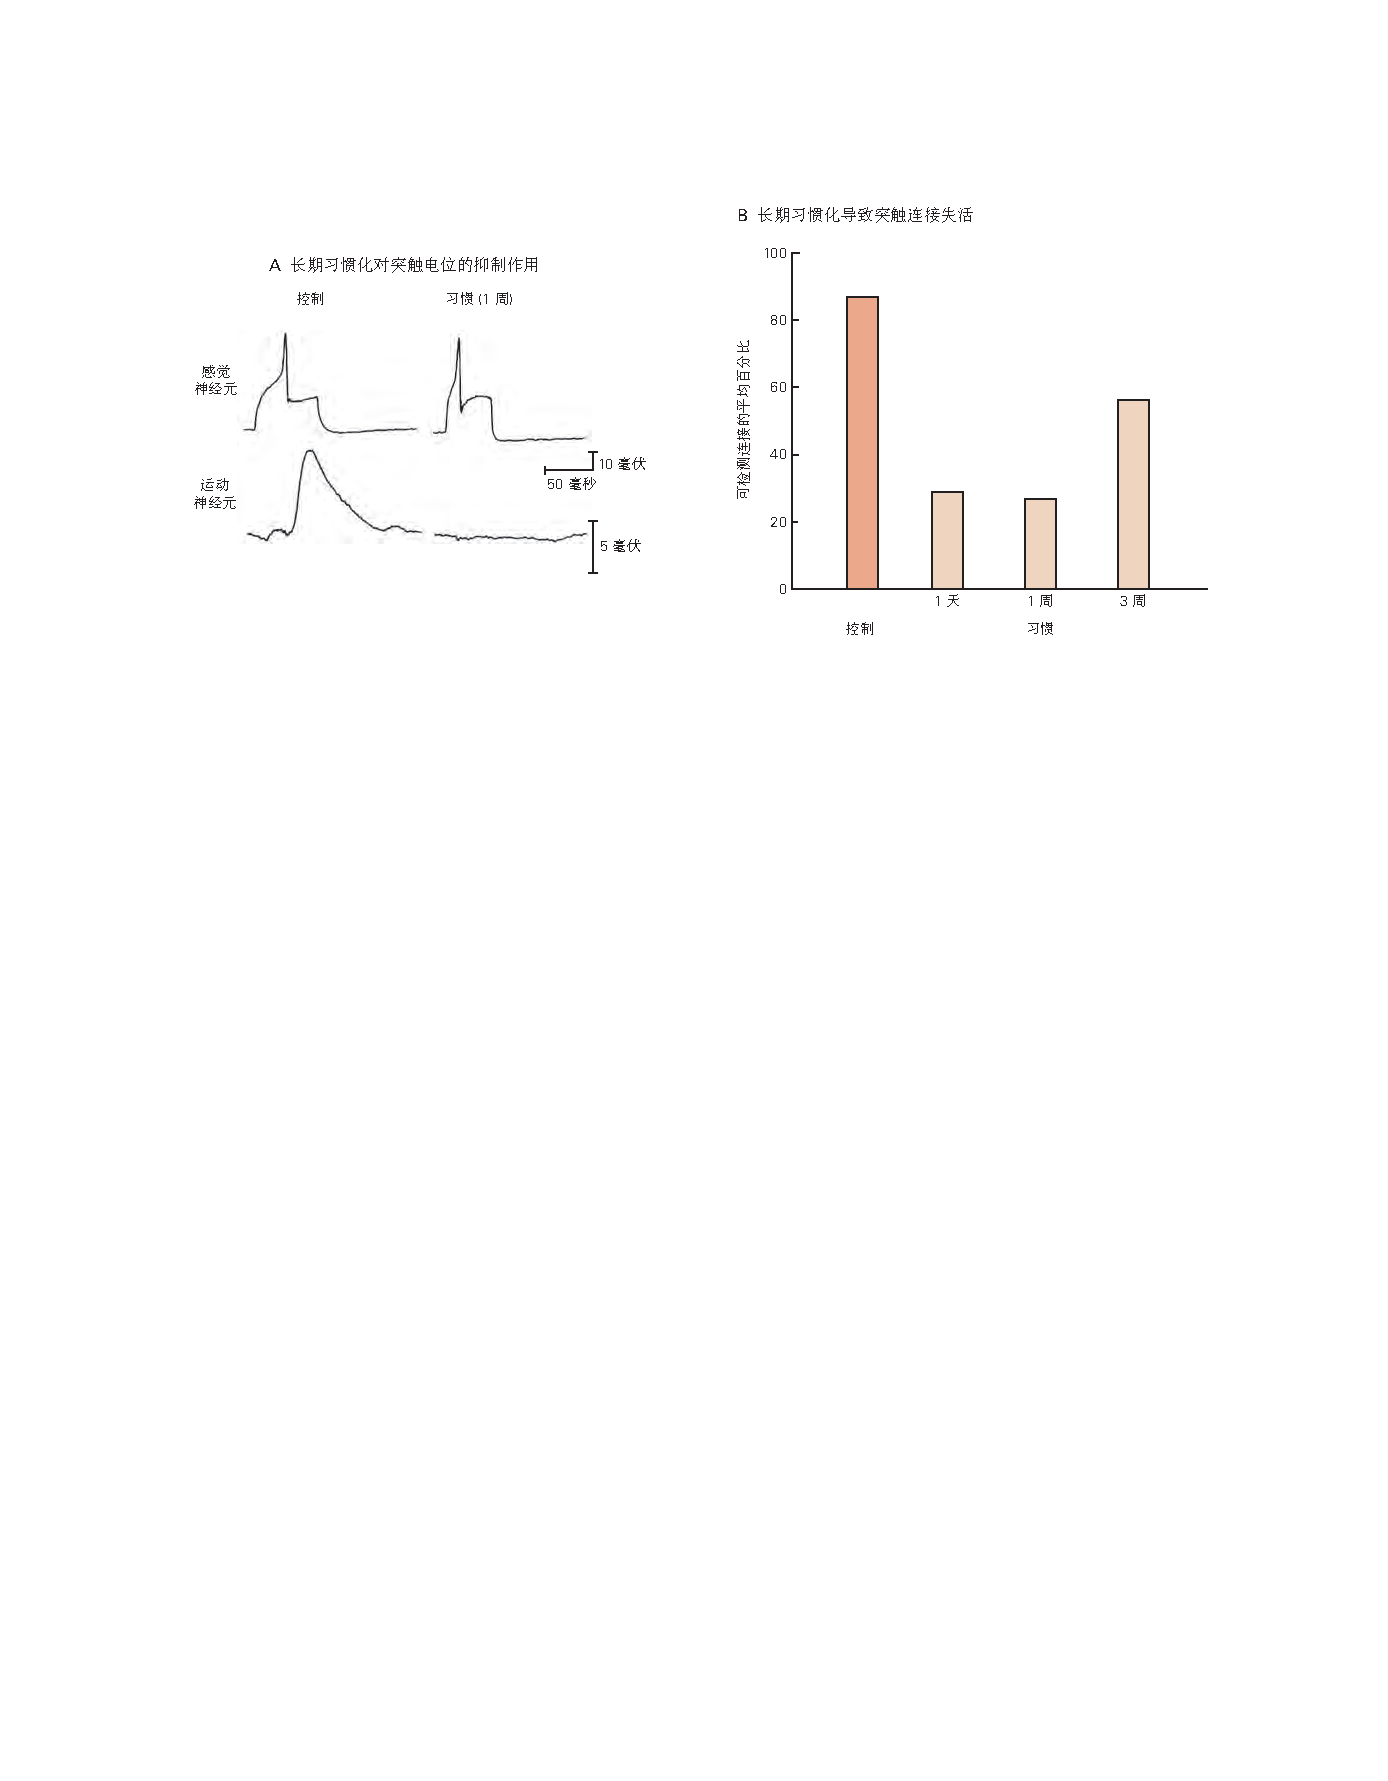
\includegraphics[width=0.85\linewidth]{chap53/fig_53_3}
	\caption{海兔\textit{缩鳃反射}的长期习惯\cite{castellucci1978cellular}。
		\textbf{A.} 未受训动物(对照)和长期习惯动物的感觉神经元动作电位和运动神经元突触后电位的比较。
		在训练后 1 周的习惯动物中,运动神经元中没有响应感觉神经元动作电位的突触电位。
		\textbf{B.} 经过长期的习惯训练,即使在 3 周时,与运动神经元建立生理可检测连接的感觉神经元的平均百分比也会降低。}
	\label{fig:53_3}
\end{figure}


解剖学研究表明,长期习惯是由感觉神经元和运动神经元之间的突触接触数量减少引起的。
在幼稚动物中,90\% 的感觉神经元与已识别的运动神经元建立生理上可检测的联系。
相比之下,在经过长期习惯训练的动物中,连接的发生率降低到 30\%;
突触数量的减少持续了一周,甚至在 3 周后也没有完全恢复(见图~\ref{fig:53_9})。
正如我们将看到的,相反的情况发生在长期敏化中,突触传递与感觉神经元和运动神经元之间突触数量的增加有关。


并非所有类别的突触都具有同等的可修改性。
在海兔中,一些突触的强度很少改变,即使反复激活也是如此。
在专门参与学习的突触中(例如\textit{缩鳃反射}回路中感觉神经元和运动神经元之间的连接),相对少量的训练可以产生突触强度的巨大而持久的变化。



\subsection{敏化涉及突触传递的突触前促进}

识别和应对危险的能力是生存所必需的。
不仅是蜗牛和苍蝇,包括人类在内的所有动物都必须区分捕食者和猎物,区分敌对环境和安全环境。
由于应对威胁的能力是生存的普遍要求,因此它在整个进化过程中一直得到保护,从而使无脊椎动物的研究能够阐明哺乳动物的神经机制。


20 世纪初,弗洛伊德和巴甫洛夫都认识到,对危险信号的预期防御反应具有生物适应性,这一事实可能解释了脊椎动物和无脊椎动物这种能力的深刻保存。
在实验室中,通常通过在厌恶刺激(例如电击)开始之前呈现中性刺激(例如音调)来研究威胁(恐惧)条件反射。
这两种刺激变得相关联,以至于音调会引发防御行为,以防止音调预测的有害后果。
弗洛伊德称这种为“信号焦虑”,即使有外部危险的暗示,它也会让个体做好战斗或逃跑的准备。


当动物反复遇到无害刺激时,它对刺激的反应会形成习惯,如上所示。
相反,当动物面临有害刺激时,它通常会学会对随后出现的相同刺激做出更强烈的反应。
有害刺激的呈现甚至可以导致动物对随后的无害刺激产生防御反应。
结果,撤退和逃跑的防御反应变得更加强烈。
这种反射反应的增强称为敏化。


像习惯一样,敏化可以是短暂的或持久的。
对海兔的尾巴进行一次电击会导致持续几分钟的\textit{缩鳃反射}的短期敏化;
对尾巴进行五次或更多次电击会产生持续数天至数周的过敏反应。
尾震也足以克服习惯化的影响并增强习惯性的\textit{缩鳃反射},这一过程称为去习惯化。


敏感化和去习惯化是由于\textit{缩鳃反射}神经回路中几个连接的突触传递增强所致,包括感觉神经元与运动神经元和中间神经元之间的连接——相同的突触被习惯化抑制(图~\ref{fig:53_4}A)。
通常,可修改的突触可以双向调节,参与不止一种类型的学习,并存储不止一种类型的记忆。
构成习惯化和敏感化基础的双向突触变化是不同细胞机制的结果。
在海兔中,通过同突触过程习惯化而被削弱的相同突触可以通过异突触过程的敏化作用得到加强,异突触过程依赖于对尾部有害刺激激活的调节性中间神经元。


\begin{figure}[htbp]
	\centering
	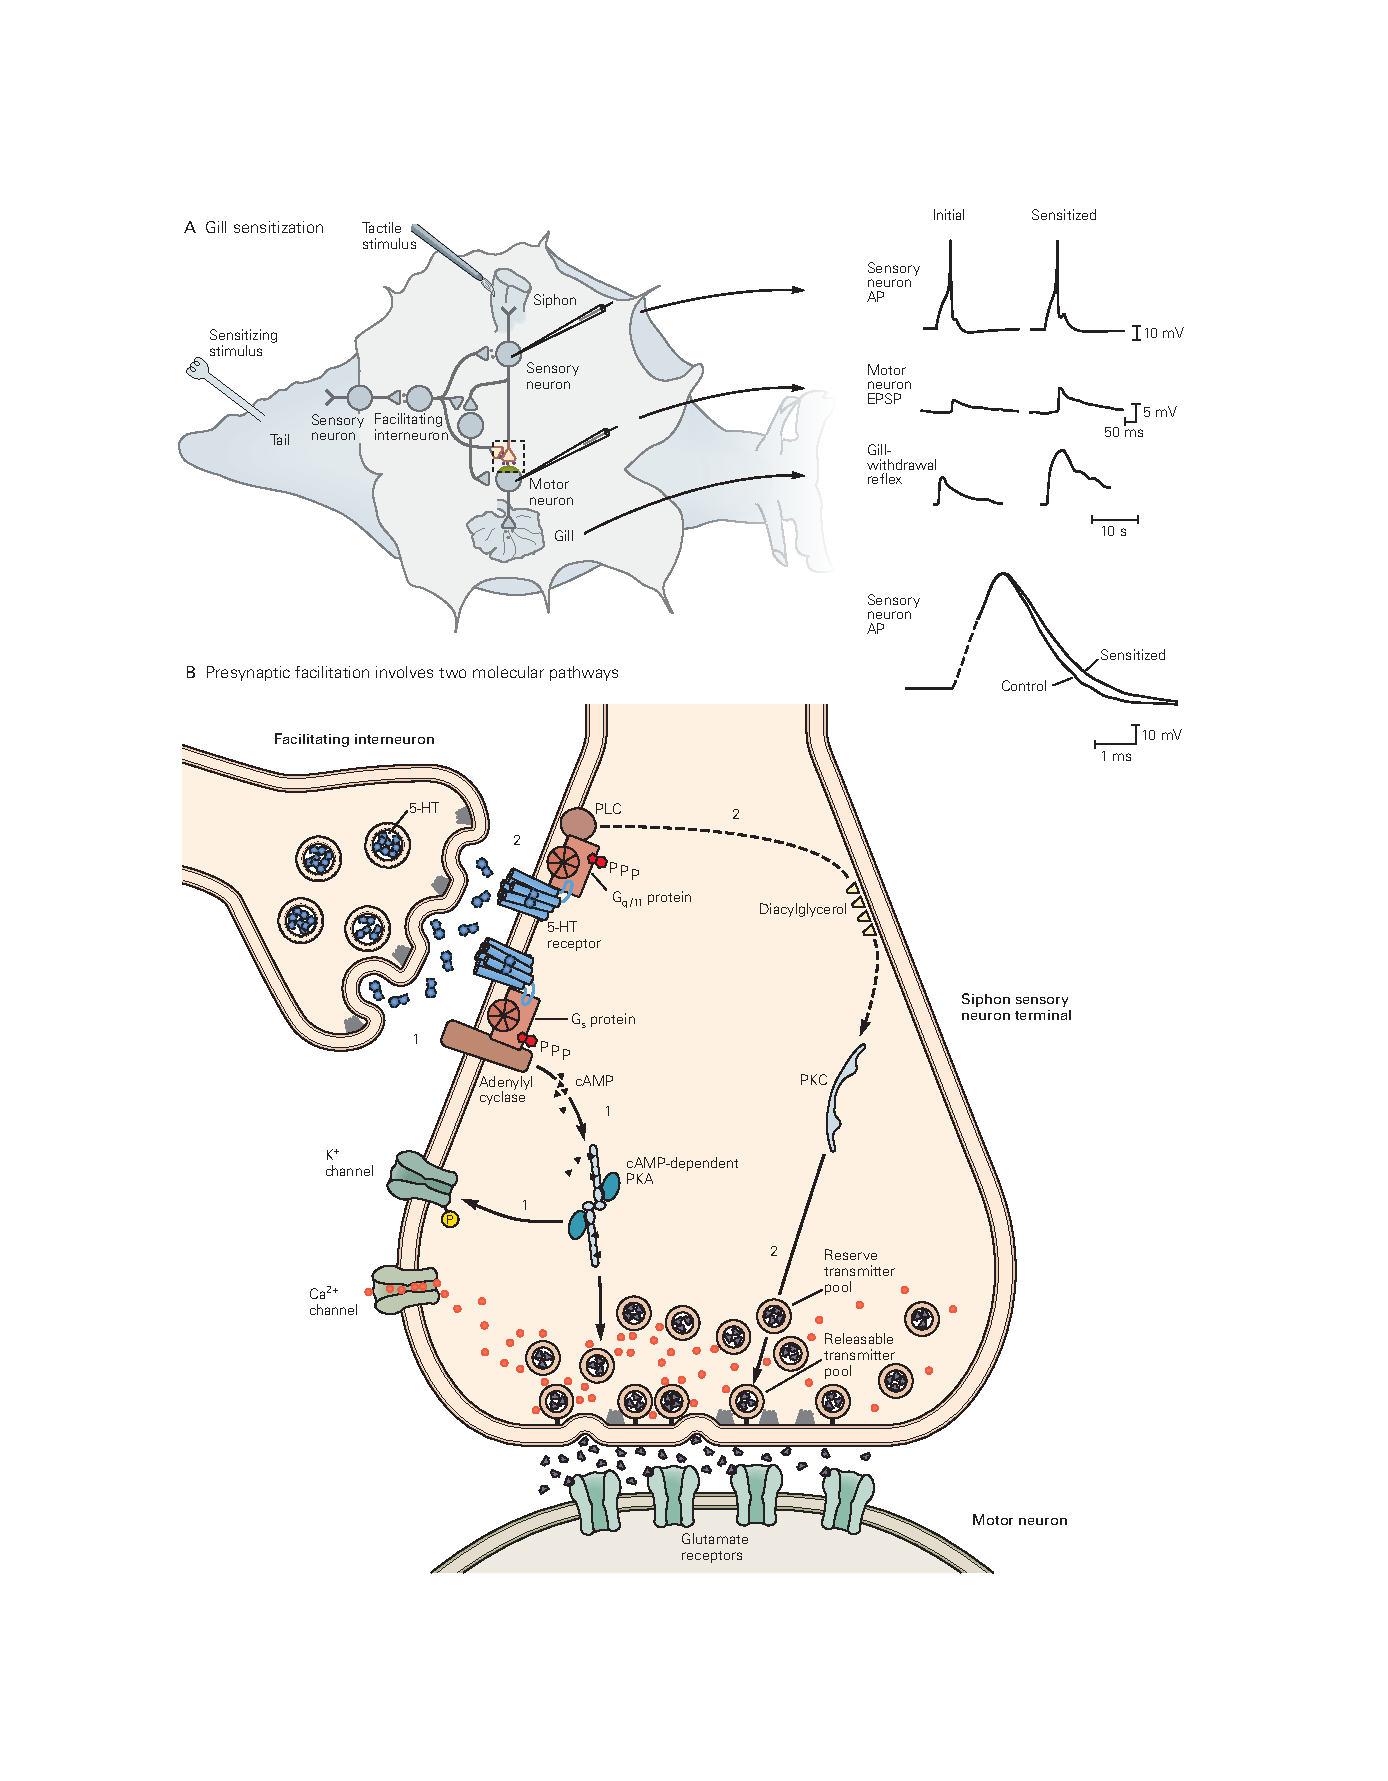
\includegraphics[width=0.9\linewidth]{chap53/fig_53_4}
	\caption{海兔\textit{缩鳃反射}的短期\textit{敏化}。
		\textbf{A.} 对身体的另一部分(例如\textit{尾巴})施加伤害性刺激会产生\textit{缩鳃反射}。
		对尾部的电击会激活尾部\textit{感觉神经元},从而激发\textit{促进}(调节)\textit{中间神经元},从而在支配\textit{虹吸管}的机械感受器感觉神经元的细胞体和末端形成突触。
		通过这些轴突-轴突突触,调节中间神经元增强递质从虹吸感觉神经元释放到它们的突触后鳃运动神经元(突触前易化),从而增强鳃退缩。
		突触前易化部分是由感觉神经元\textit{动作电位}(底部轨迹)的延长引起的\cite{pinsker1970habituation,klein1980mechanism}。
		\textbf{B.} 感觉神经元中的突触前易化作用被认为是通过两种生化途径发生的。
		该图在 A 部分的虚线框中显示了突触复合体的详细信息。
		\textit{通路 1}:促进中间神经元释放\textit{5-羟基色氨酸},它与感觉神经元末梢的促代谢受体结合。
		该作用与 G 蛋白 ($ G_s $) 结合,进而增加\textit{腺苷酸环化酶}的活性。
		腺苷酸环化酶将\textit{三磷酸腺苷}转化为\textit{环磷酸腺苷},后者与\textit{蛋白激酶A}的调节亚基结合,从而激活其催化亚基。
		催化亚基磷酸化某些 \ce{K+} 通道,从而关闭通道并减少向外的 \ce{K+} 电流。
		这会延长动作电位,从而增加 \ce{Ca^2+} 通过电压门控 \ce{Ca^2+} 通道的流入,从而增加递质释放。
		\textit{通路 2}:\textit{5-羟基色氨酸}与第二类促代谢受体结合,后者激活 G 蛋白的 $ G_{q/11} $ 类,从而增强\textit{磷脂酶C}的活性。
		\textit{磷脂酶C}活性导致\textit{甘油二酯}的产生,从而激活\textit{蛋白激酶C}。
		\textit{蛋白激酶C}磷酸化突触前蛋白,导致含有谷氨酸的囊泡从\textit{储备池}动员到活性区的\textit{可释放池},从而提高递质释放的效率。}
	\label{fig:53_4}
\end{figure}


至少三组调节中间神经元参与敏化。
研究最充分的是使用血清素作为递质(图~\ref{fig:53_4}B)。
5-羟色胺能中间神经元在感觉神经元的许多区域形成突触,包括感觉细胞突触前末端的轴突-轴突突触。
在单次尾部电击后,从中间神经元释放的血清素与感觉神经元中的受体结合,该受体与刺激性 G 蛋白偶联,从而增加腺苷酸环化酶的活性。
该作用产生第二信使\textit{环磷酸腺苷},后者又激活\textit{环磷酸腺苷}依赖性\textit{蛋白激酶A}(第~\ref{chap:chap14}~章)。
5-羟色胺还激活第二种类型的 G 蛋白偶联受体,导致磷脂水解和\textit{蛋白激酶C}激活。


由\textit{蛋白激酶A}和\textit{蛋白激酶C}介导的蛋白质磷酸化通过至少两种机制增强感觉神经元递质的释放(图~\ref{fig:53_4}B)。
在一个动作中,\textit{蛋白激酶A}磷酸化 \ce{K+} 通道,使其关闭。 这拓宽了动作电位,从而延长了 \ce{Ca^2+} 通过电压门控 \ce{Ca^2+} 通道流入的持续时间,进而增强了递质释放。
在第二个作用中,通过\textit{蛋白激酶C}的蛋白质磷酸化直接增强了释放机制的功能。
响应尾部电击释放血清素的突触前易化作用持续数分钟。
反复的伤害性刺激可以在数天之内增强突触活动(通过我们在下面考虑的机制)。



\subsection{经典威胁条件反射涉及促进突触传递}

经典条件反射是一种更复杂的学习形式。
动物学习将一种类型的刺激与另一种类型的刺激联系起来,而不是像在习惯化和敏感化中那样学习一种刺激的特性。
如第~\ref{chap:chap52}~章所述,当与强烈的非条件刺激(例如,提供食物)配对时,最初的弱条件刺激(例如,铃声)在产生反应方面变得非常有效。
在可以通过经典条件反射和敏化作用增强的反射中,例如海兔的防御性\textit{缩鳃反射},经典条件反射会导致更大和更持久的增强。


尽管厌恶经典条件反射传统上被称为恐惧条件反射,但我们将使用更中性的术语威胁条件反射来避免暗示动物具有与人类经历和标记为“恐惧”的主观状态相当的主观状态。 这种区别很重要,因为人类可以在没有任何报告的恐惧感的情况下在行为和生理上对威胁做出反应。
这个术语允许以客观的方式解释所有动物(从最简单的蠕虫到人类)内隐学习的研究结果,而无需在动物中援引经验上无法验证的主观恐惧状态。


对于海兔\textit{缩鳃反射}的经典条件反射,对虹吸管的微弱触摸作为条件刺激,而对尾巴的强烈冲击作为非条件刺激。
当\textit{缩鳃反射}受到经典条件反射时,单独对虹吸刺激的反应大大增强。
这种增强甚至比单独通过尾部电击(致敏)在未配对通路中产生的增强更为显着。 
在经典条件反射中,条件刺激和非条件刺激的时间安排至关重要。
为了有效,条件刺激(虹吸式触摸)必须先于(并因此预测)非条件刺激(尾震),通常间隔约 0.5 秒。


由条件刺激和非条件刺激引发的信号在单个感觉神经元中的收敛是至关重要的。
独自一人,对尾巴的强烈冲击(无条件刺激)将激发 5-羟色胺能中间神经元,在虹吸感觉神经元的突触前末端形成突触,从而导致突触前易化(图~\ref{fig:53_5}A)。
然而,当轻微敲击虹吸管(条件刺激)后立即发生尾部电击时,来自中间神经元的血清素会产生更大的突触前易化作用,这一过程称为活动依赖性易化作用(图~\ref{fig:53_5}B)。


\begin{figure}[htbp]
	\centering
	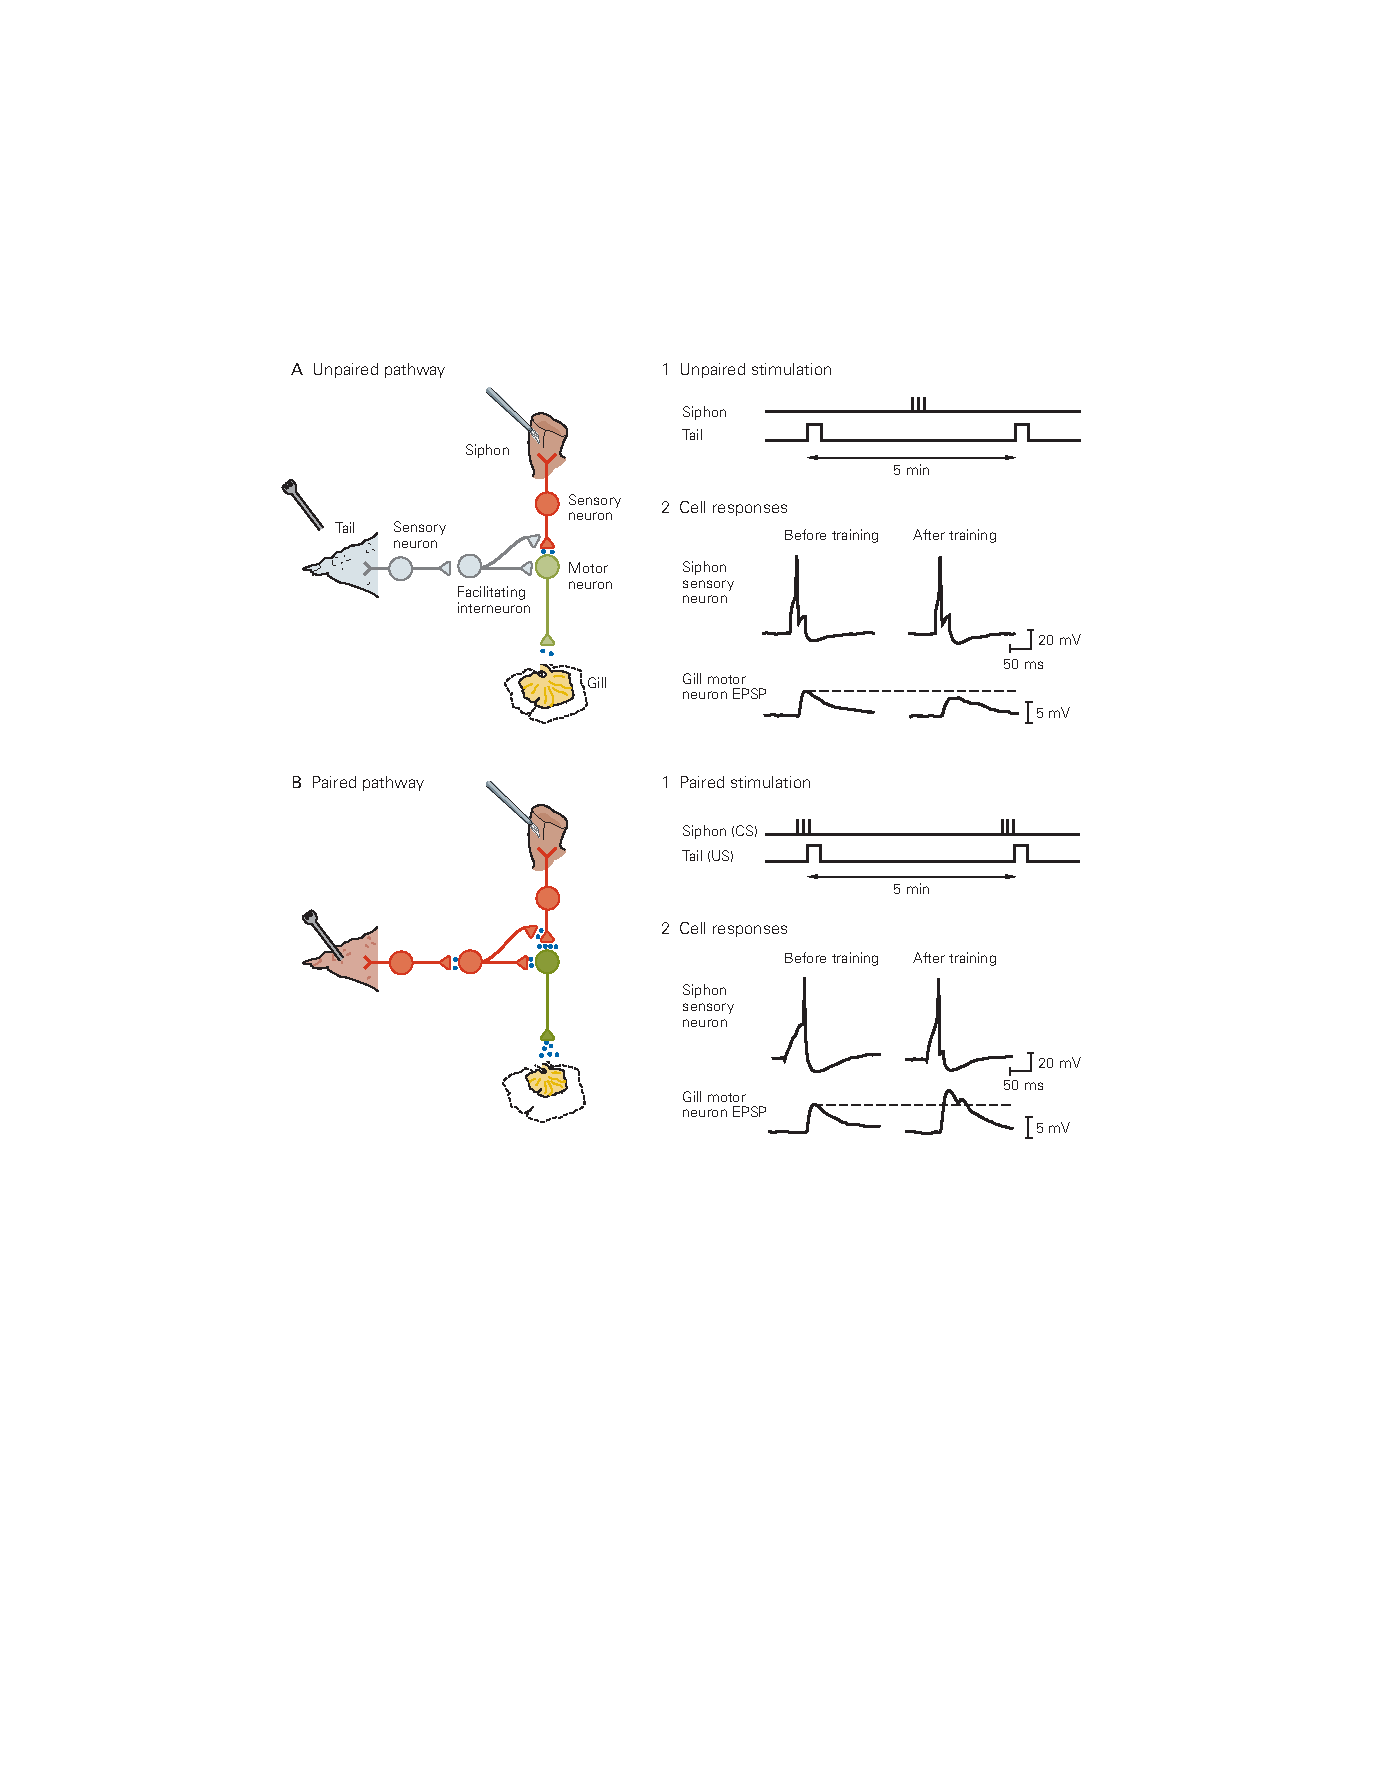
\includegraphics[width=0.9\linewidth]{chap53/fig_53_5}
	\caption{海兔\textit{缩鳃反射}的经典调节\cite{hawkins1983cellular}。
		\textbf{A.} 虹吸管受到轻敲刺激,尾巴受到电击,但两种刺激没有及时配对。
		尾震激发易化中间神经元,在感觉神经元的突触前末端形成突触,支配地幔架和虹吸管。
		这就是致敏机制。
		1.训练过程中不成对刺激的模式。
		2. 在这些条件下,运动神经元测试\textit{兴奋性突触后电位}的大小仅受尾部电击的微弱影响。
		通常,如本例所示,尽管存在尾部电击,但\textit{兴奋性突触后电位}实际上会略有下降,因为虹吸管的重复不成对刺激会因习惯而导致突触抑制。
		\textbf{B.} 尾震与虹吸管的刺激及时配对。
		1. 在电击尾巴(\textit{非条件刺激})之前立即触摸虹吸管(\textit{条件刺激})。
		结果,虹吸管感觉神经元准备好对来自无条件通路中的易化中间神经元的输入更敏感。
		这是经典条件反射的机制;
		它选择性地放大条件通路的反应。
		2. 在训练前和训练后 1 小时由虹吸感觉神经元产生的已识别运动神经元中测试\textit{兴奋性突触后电位}的记录。
		在使用配对感觉输入进行训练后,虹吸运动神经元中的\textit{兴奋性突触后电位}比训练前的\textit{兴奋性突触后电位}或未配对的尾部电击后的\textit{兴奋性突触后电位}大得多(如 A2 部分所示)。
		这种突触放大会产生更有力的鳃收缩。}
	\label{fig:53_5}
\end{figure}


这是如何运作的?
在调节过程中,在虹吸管感觉神经元中通过敲击虹吸管产生动作电位后不久,由尾震激活的调节性中间神经元释放血清素。
动作电位触发 \ce{Ca^2+} 流入感觉神经元的突触前末梢,\ce{Ca^2+} 与钙调蛋白结合,钙调蛋白又与腺苷酸环化酶结合。
这启动了腺苷酸环化酶,使其对尾部休克后释放的血清素反应更加强烈。
这反过来又增强了\textit{环磷酸腺苷}的产生,从而增加了突触前易化作用的量。
如果颠倒刺激顺序,使血清素释放先于 \ce{Ca^2+} 流入突触前感觉末梢,则没有增强作用,也没有经典条件作用。


因此,戒断反射的单突触通路中经典调节的细胞机制主要是对致敏机制的详细阐述,其附加特征是腺苷酸环化酶在突触前感觉神经元中充当巧合检测器,识别 对尾部冲击(无条件刺激)和虹吸龙头(条件刺激)的生理反应。


除了活动依赖性易化的突触前成分外,当虹吸管感觉神经元高度兴奋时,突触后成分由 \ce{Ca^2+} 流入运动神经元触发。
这种突触后机制的特性类似于哺乳动物大脑中突触传递的长期增强(在本章后面以及第~\ref{chap:chap13}~章和第~\ref{chap:chap54}~章中讨论)。



\section{内隐记忆的长期存储涉及由\textit{环磷酸腺苷}-\textit{蛋白激酶A}-\textit{环磷酸腺苷应答元件结合蛋白}通路介导的突触变化}

\subsection{\textit{环磷酸腺苷}信号在长期致敏中起作用}

在所有形式的学习中,熟能生巧。
重复的经验将短期记忆转化为长期形式。
在海兔中,最深入研究的长期记忆形式是长期敏化。
与短期形式一样,\textit{缩鳃反射}的长期敏化涉及多个突触连接强度的变化。
但除此之外,它还招募了新的突触连接的增长。


大约 1 小时的五次间隔训练课程(或重复应用血清素)会产生持续 1 天或更长时间的长期敏化和长期突触促进。
几天的间隔训练会产生持续 1 周或更长时间的敏化。
长期致敏与短期致敏一样,需要依赖于增加的\textit{环磷酸腺苷}水平的蛋白质磷酸化(图~\ref{fig:53_6})。


\begin{figure}[htbp]
	\centering
	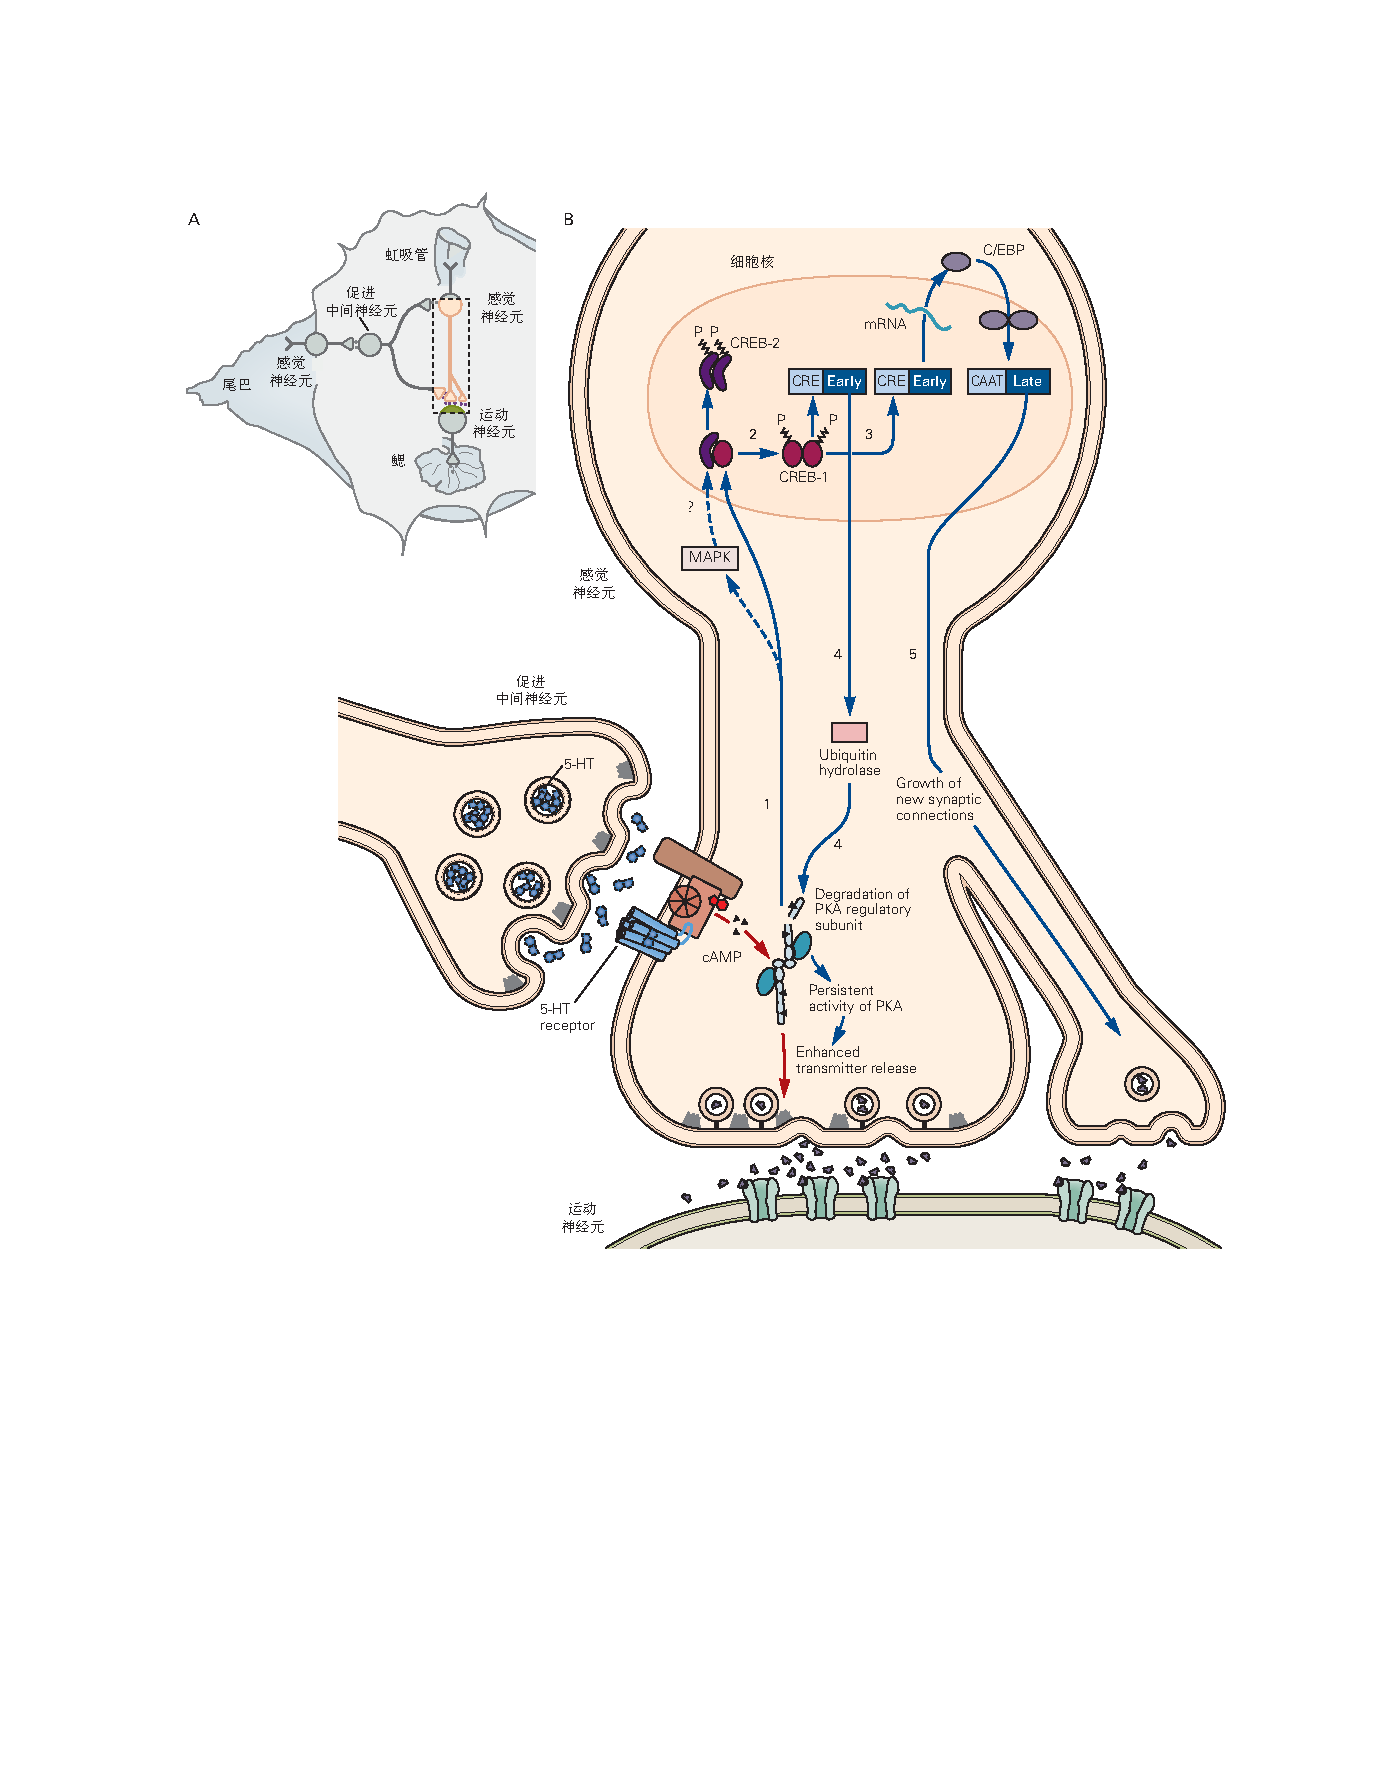
\includegraphics[width=1.0\linewidth]{chap53/fig_53_6}
	\caption{长期致敏涉及突触促进和新突触连接的增长。
		\textbf{A.} 海兔的\textit{缩鳃反射}的长期敏感化涉及在感觉神经元和运动神经元之间的突触处持久促进递质释放。
		\textbf{B.} \textit{缩鳃反射}的长期敏感导致\textit{蛋白激酶A}的持续活性,导致新突触连接的生长。
		重复的尾部休克导致\textit{环磷酸腺苷}更明显的升高,产生长期促进作用(持续 1 天或更长时间),其持续时间超过\textit{环磷酸腺苷}的增加并募集新蛋白质的合成。
		这种诱导机制由\textit{蛋白激酶A}易位至细胞核(通路 1)启动,其中\textit{蛋白激酶A}磷酸化转录激活因子\textit{环磷酸腺苷}反应元件结合蛋白 1 (\textit{环磷酸腺苷应答元件结合蛋白}-1)(途径 2)。
		\textit{环磷酸腺苷应答元件结合蛋白}-1 结合位于几个\textit{环磷酸腺苷}诱导基因上游区域的\textit{环磷酸腺苷应答元件},激活基因转录(通路 3)。
		\textit{蛋白激酶A}还激活\textit{有丝分裂原活化蛋白激酶},后者磷酸化转录抑制因子\textit{环磷酸腺苷}反应元件结合蛋白 2 (\textit{环磷酸腺苷应答元件结合蛋白}-2),从而消除其抑制作用。
		\textit{环磷酸腺苷应答元件结合蛋白}-1 激活的一个基因编码一种泛素水解酶,它是一种特定泛素蛋白酶体的一种成分,可导致\textit{蛋白激酶A}调节亚基的蛋白水解裂解,从而导致\textit{蛋白激酶A}的持续活性,即使在\textit{环磷酸腺苷}恢复到其静止水平后(通路 4)。
		\textit{环磷酸腺苷应答元件结合蛋白}-1 还激活转录因子 C/EBP 的表达,从而导致一组未鉴定的蛋白质的表达,这些蛋白质对新突触连接的生长很重要(通路 5)。}
	\label{fig:53_6}
\end{figure}


将短期记忆转化为长期记忆,称为巩固,需要在回路中的神经元中合成\textit{信使核糖核酸}和蛋白质。
因此,长期记忆需要特定基因表达的激活。
从短期记忆到长期记忆的转变取决于重复使用血清素后\textit{环磷酸腺苷}的持续升高。
\textit{环磷酸腺苷}的增加导致\textit{蛋白激酶A}的激活时间延长,从而使激酶的催化亚基转移到感觉神经元的细胞核中。
它还间接导致第二种蛋白激酶的激活,即\textit{有丝分裂原活化蛋白激酶},这是一种通常与细胞生长相关的激酶(第~\ref{chap:chap14}~章)。
在细胞核内,\textit{蛋白激酶A}的催化亚基磷酸化,从而激活转录因子 \textit{环磷酸腺苷应答元件结合蛋白}-1(\textit{环磷酸腺苷} 反应元件结合蛋白 1),它结合称为\textit{环磷酸腺苷应答元件}(识别元件)的启动子元件(图~\ref{fig:53_6}~和~\ref{fig:53_7}) 。


\begin{figure}[htbp]
	\centering
	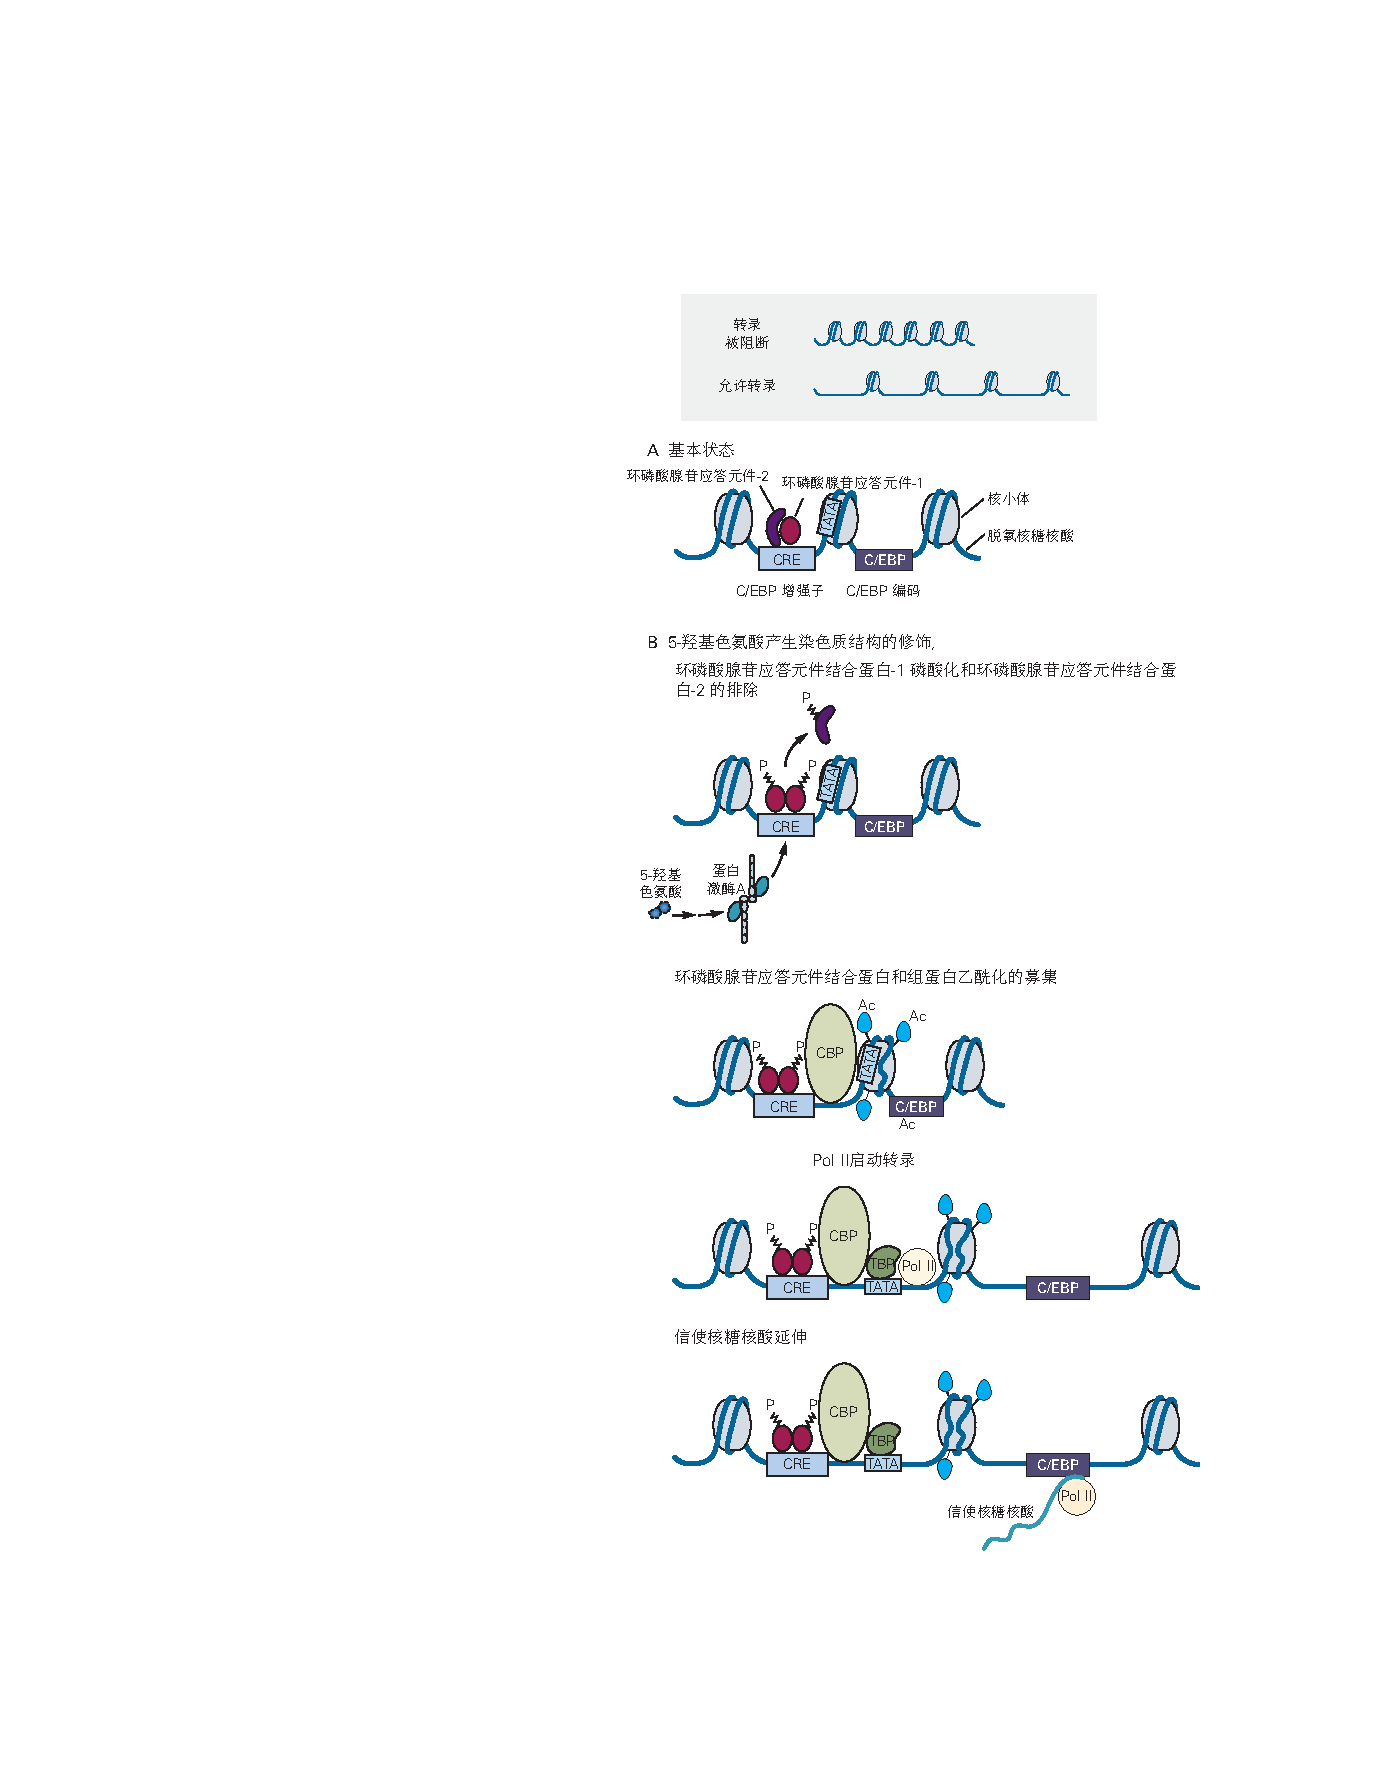
\includegraphics[width=0.6\linewidth]{chap53/fig_53_7}
	\caption{血清素、\textit{环磷酸腺苷应答元件结合蛋白}-1 和\textit{环磷酸腺苷应答元件结合蛋白}对组蛋白乙酰化的调节。 
		\textbf{A.} 在基础条件下,激活剂 \textit{环磷酸腺苷应答元件结合蛋白}-1(此处与 \textit{环磷酸腺苷应答元件结合蛋白}-2 复合)占据其靶基因启动子区域内\textit{环磷酸腺苷应答元件}的结合位点。
		在此处显示的示例中,\textit{环磷酸腺苷应答元件结合蛋白}-1 与 C/EBP 启动子内的\textit{环磷酸腺苷应答元件}结合。
		在基础状态下,\textit{环磷酸腺苷应答元件结合蛋白}-1 结合无法激活转录,因为 TATA 盒是转录起始期间负责募集\textit{核糖核酸}聚合酶 II (Pol II) 的核心启动子区域,无法进入,因为\textit{脱氧核糖核酸}与组蛋白紧密结合核小体。
		\textbf{B.} \textit{5-羟基色氨酸}激活\textit{蛋白激酶A},使 \textit{环磷酸腺苷应答元件结合蛋白}-1 磷酸化并通过 \textit{有丝分裂原活化蛋白激酶} 间接增强 \textit{环磷酸腺苷应答元件结合蛋白}-2 磷酸化,导致 \textit{环磷酸腺苷应答元件结合蛋白}-2 从启动子上解离。
		这允许 \textit{环磷酸腺苷应答元件结合蛋白}-1 在启动子处与 \textit{环磷酸腺苷应答元件结合蛋白} 结合蛋白形成复合物。
		活化的\textit{环磷酸腺苷应答元件结合蛋白}乙酰化组蛋白的特定赖氨酸残基,导致它们与\textit{脱氧核糖核酸}的结合不那么紧密。
		随着染色质结构的其他变化,乙酰化有助于核小体的重新定位,该核小体先前阻止了 Pol II 复合物进入 TATA 盒。
		这种重新定位允许招募 Pol II 以启动 C/EBP 基因的转录。}
	\label{fig:53_7}
\end{figure}


为了启动基因转录,磷酸化的 \textit{环磷酸腺苷应答元件结合蛋白}-1 将转录共激活因子\textit{环磷酸腺苷应答元件结合蛋白}结合蛋白募集到启动子区域。
\textit{环磷酸腺苷应答元件结合蛋白}具有促进转录激活的两个重要特性:它将\textit{核糖核酸}聚合酶 II 募集到启动子,并且它作为乙酰转移酶发挥作用,将乙酰基添加到其底物蛋白上的某些赖氨酸残基。
\textit{环磷酸腺苷应答元件结合蛋白}最重要的底物之一是\textit{脱氧核糖核酸}结合组蛋白,它是核小体的成分,是染色质的基本组成部分。
组蛋白包含一系列带正电荷的碱性残基,这些残基与带负电荷的\textit{脱氧核糖核酸}磷酸盐发生强烈相互作用。
这种相互作用导致\textit{脱氧核糖核酸}紧紧包裹在核小体周围,就像线缠绕在线轴上一样,从而阻止必要的转录因子接近其基因靶标。


\textit{环磷酸腺苷应答元件结合蛋白}与\textit{环磷酸腺苷应答元件结合蛋白}-1 的结合会导致组蛋白乙酰化,从而在核小体水平引起许多重要的结构和功能变化。
例如,乙酰化中和了组蛋白尾区赖氨酸残基的正电荷,降低了组蛋白对\textit{脱氧核糖核酸}的亲和力。
此外,特定类别的转录激活剂可以与乙酰化组蛋白结合并促进核小体在启动子区域的重新定位。 这些和其他类型的染色质修饰一起用于调节染色质对转录机制的可及性,从而增强基因的转录能力。
这种类型的\textit{脱氧核糖核酸}结构修饰称为表观遗传调控。
正如我们将在第~\ref{chap:chap54}~章中看到的,编码\textit{环磷酸腺苷应答元件结合蛋白}的基因突变是鲁宾斯坦-泰比综合征的基础,这是一种与智力低下相关的疾病。


\textit{蛋白激酶A}启动转录还取决于其间接激活 \textit{有丝分裂原活化蛋白激酶} 通路的能力(第~\ref{chap:chap14}~章)。
\textit{有丝分裂原活化蛋白激酶} 磷酸化转录因子 \textit{环磷酸腺苷应答元件结合蛋白}-2,解除其对转录的抑制作用(图~\ref{fig:53_6}B)。
\textit{环磷酸腺苷应答元件结合蛋白}-1 激活和\textit{环磷酸腺苷应答元件结合蛋白}-2 抑制缓解的联合作用会诱导一系列对学习和记忆很重要的新基因表达(图~\ref{fig:53_7})。


在长期促进的第一步中同时存在转录抑制因子 (\textit{环磷酸腺苷应答元件结合蛋白}-2) 和转录激活因子 (\textit{环磷酸腺苷应答元件结合蛋白}-1) 表明可以调节长期记忆存储的阈值。
事实上,我们在日常生活中看到,短期记忆转化为长期记忆的难易程度随注意力、情绪和社会背景的不同而有很大差异。



\subsection{非编码\textit{核糖核酸}在转录调控中的作用}

除了\textit{信使核糖核酸},记忆巩固和再巩固中还有其他转录和染色质调节目标。
特别感兴趣的是非编码\textit{核糖核酸},例如\textit{微小核糖核酸}、\textit{与Piwi蛋白相作用的核糖核酸}和长链非编码\textit{核糖核酸}。
这些也针对特定的遗传位点,它们的表达反过来调节转录和转录后机制。


对海兔的研究表明,\textit{微小核糖核酸}和\textit{与Piwi蛋白相作用的核糖核酸}均受神经元活动调节,并有助于长期促进。
微小\textit{核糖核酸}是一类保守的非编码\textit{核糖核酸},长度为 20 到 23 个核苷酸,通过一组特定的\textit{核糖核酸}-蛋白质机制促进基因表达的转录和转录后调控。
在海兔中,这些\textit{微小核糖核酸}中最丰富和最保守的大脑种类存在于感觉神经元中,其中之一——\textit{微小核糖核酸}-124——通常通过抑制 \textit{环磷酸腺苷应答元件结合蛋白}-1 \textit{信使核糖核酸}的翻译、抑制\textit{环磷酸腺苷应答元件结合蛋白}-1 蛋白的水平来限制血清素诱导的突触促进。
血清素抑制 \textit{微小核糖核酸}-124 的合成,从而导致 \textit{环磷酸腺苷应答元件结合蛋白}-1 \textit{信使核糖核酸} 翻译的去抑制,从而启动\textit{环磷酸腺苷应答元件结合蛋白}-1 介导的转录。
\textit{与Piwi蛋白相作用的核糖核酸}的长度为 28 到 32 个核苷酸,比\textit{微小核糖核酸}稍长,并与一种叫做 Piwi 的蛋白质结合。
单个\textit{与Piwi蛋白相作用的核糖核酸}促进特定\textit{脱氧核糖核酸}序列的甲基化,从而沉默基因,提供表观遗传调控的另一个例子。
一种\textit{与Piwi蛋白相作用的核糖核酸},\textit{与Piwi蛋白相作用的核糖核酸}-F,增加对血清素的反应,导致\textit{环磷酸腺苷应答元件结合蛋白}-2 启动子的甲基化,减少\textit{环磷酸腺苷应答元件结合蛋白}-2 基因转录。


因此,我们在这里看到了转录水平整合作用的一个例子。
5-羟色胺以协调的方式调节\textit{与Piwi蛋白相作用的核糖核酸}和\textit{微小核糖核酸}:5-羟色胺迅速降低\textit{微小核糖核酸}-124 的水平并促进\textit{环磷酸腺苷应答元件结合蛋白}-1 的激活,从而开始记忆巩固过程。
延迟后,血清素还会增加\textit{与Piwi蛋白相作用的核糖核酸}-F 的水平,导致转录抑制因子\textit{环磷酸腺苷应答元件结合蛋白}-2 的启动子甲基化和沉默。
\textit{环磷酸腺苷应答元件结合蛋白}-2 的减少增加了\textit{环磷酸腺苷应答元件结合蛋白}-1 的作用持续时间,从而巩固了感觉神经元中长期记忆的稳定形式(图~\ref{fig:53_8})。


\begin{figure}[htbp]
	\centering
	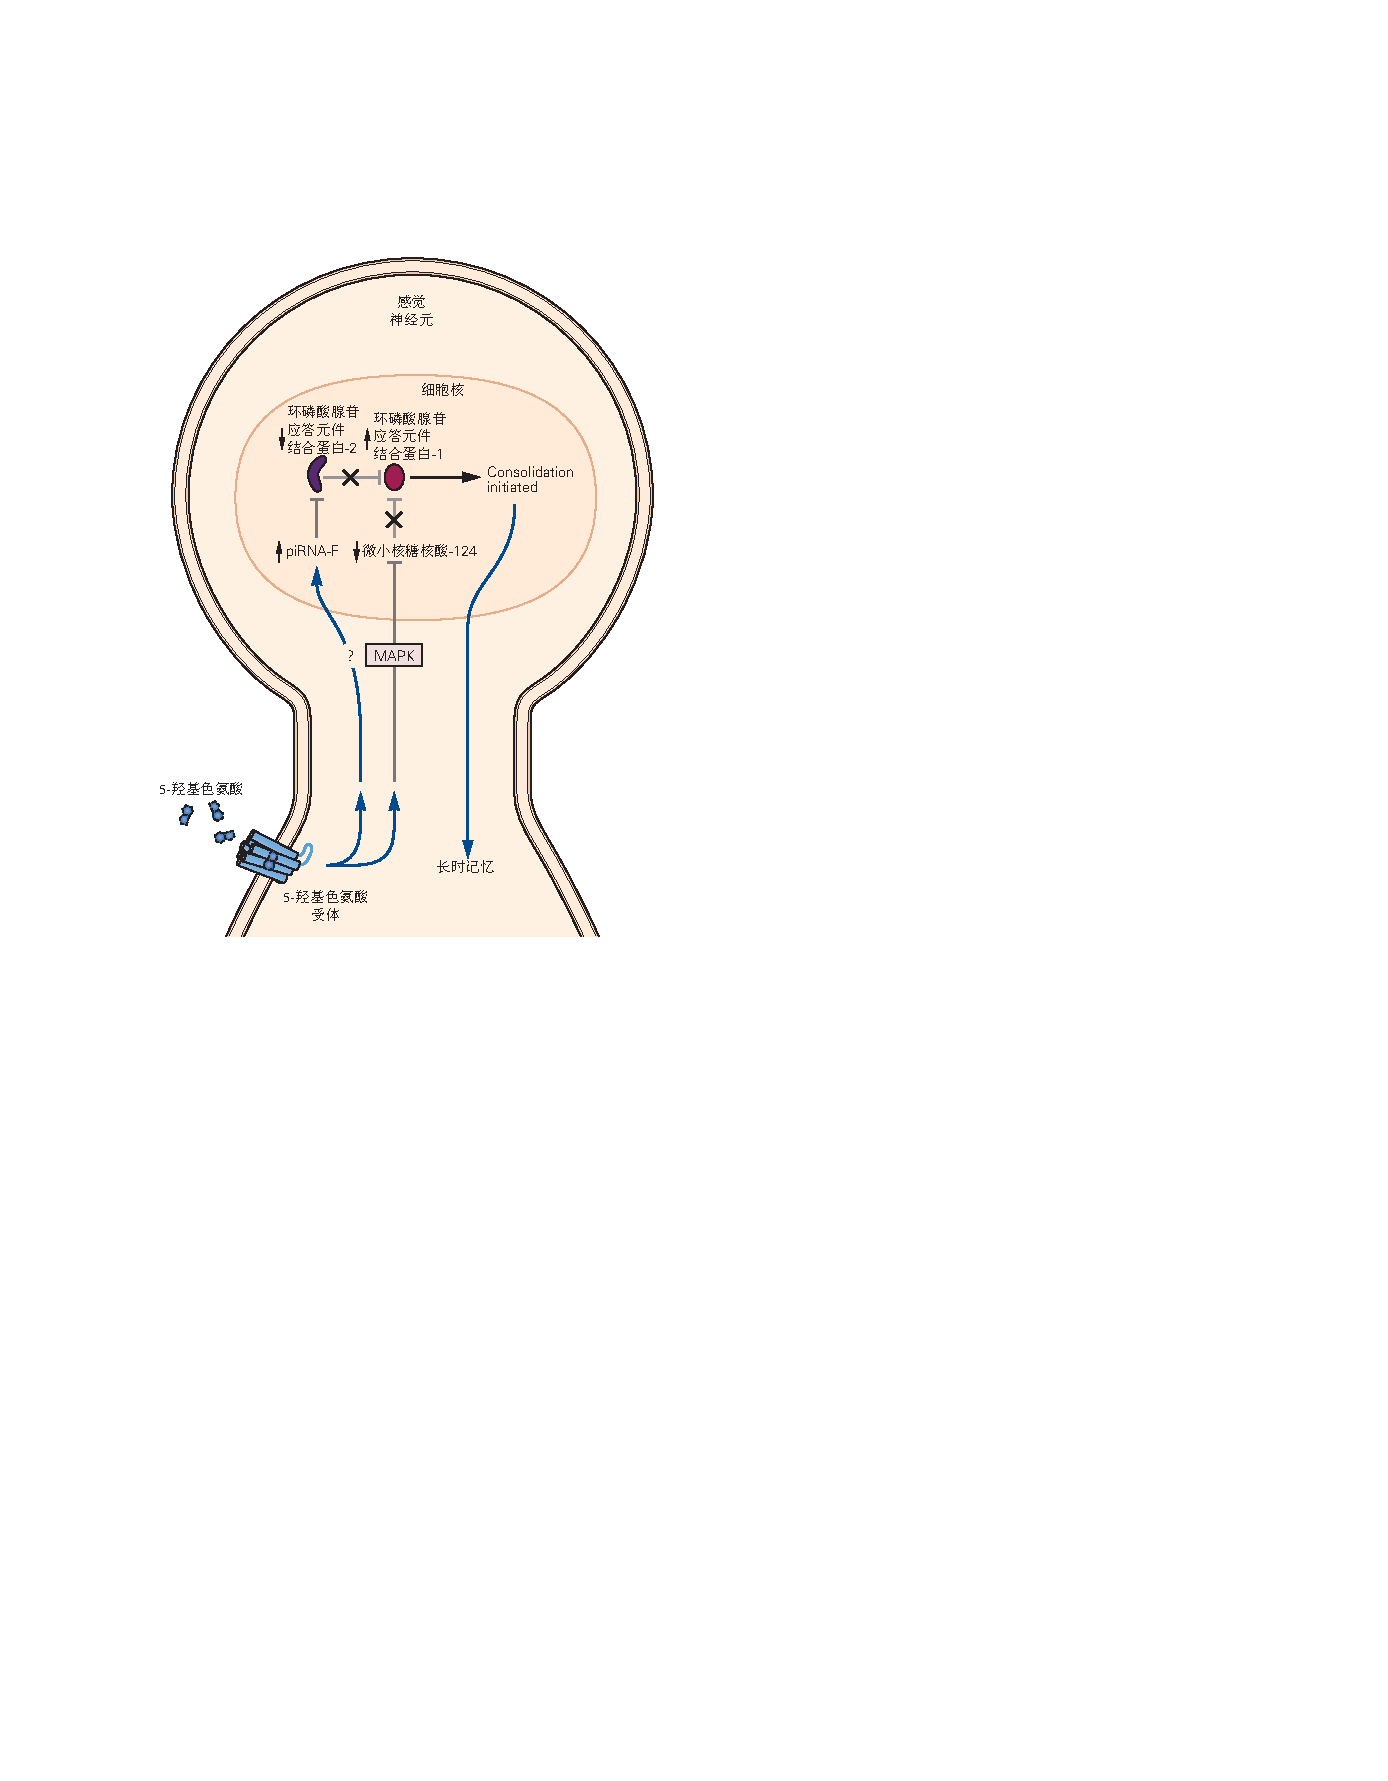
\includegraphics[width=0.55\linewidth]{chap53/fig_53_8}
	\caption{小的非编码\textit{核糖核酸}分子有助于记忆巩固开关。
		通过两种不同类别的小非编码\textit{核糖核酸}分子的作用,巩固了感觉运动神经元突触的长期促进作用。
		\textit{微小核糖核酸}-124 通常通过与其\textit{信使核糖核酸}结合并抑制其翻译来抑制\textit{环磷酸腺苷应答元件结合蛋白}-1 转录因子的水平。
		\textit{5-羟基色氨酸}通过需要\textit{有丝分裂原活化蛋白激酶}的机制下调 \textit{微小核糖核酸}-124 水平。
		这提高了 \textit{环磷酸腺苷应答元件结合蛋白}-1 的水平,促进了记忆巩固所必需的基因产物的 \textit{环磷酸腺苷应答元件结合蛋白}-1 依赖性转录的激活。
		在互补途径中,5-HT 增强并延迟了几种\textit{与Piwi蛋白相作用的核糖核酸}的合成,包括与 Piwi 蛋白结合的\textit{与Piwi蛋白相作用的核糖核酸}-F。
		\textit{与Piwi蛋白相作用的核糖核酸}-F/Piwi 复合物导致\textit{环磷酸腺苷应答元件结合蛋白}-2 基因的甲基化增强,导致\textit{环磷酸腺苷应答元件结合蛋白}-2 的长期转录抑制和\textit{环磷酸腺苷应答元件结合蛋白}-2 蛋白水平降低。
		由于\textit{环磷酸腺苷应答元件结合蛋白}-2 通常会抑制\textit{环磷酸腺苷应答元件结合蛋白}-1 的作用,因此响应\textit{5-羟基色氨酸}的 \textit{与Piwi蛋白相作用的核糖核酸}-F 水平增加会增强和延长\textit{环磷酸腺苷应答元件结合蛋白}-1 活性,从而导致更有效的记忆巩固。}
	\label{fig:53_8}
\end{figure}


在\textit{环磷酸腺苷应答元件结合蛋白}-1 激活后表达的两个基因和随之而来的染色质结构改变在长期促进的早期发展中很重要。
一个是泛素羧基末端水解酶基因,另一个是转录因子基因,CAAT 盒增强子结合蛋白 (C/EBP),是合成新突触连接生长所需蛋白质所必需的基因级联的组成部分(图~\ref{fig:53_6}和\ref{fig:53_7})。


水解酶促进泛素介导的蛋白质降解(第~\ref{chap:chap7}~章)并有助于增强\textit{蛋白激酶A}的激活。
\textit{蛋白激酶A}由四个亚基组成;
两个调节亚基抑制两个催化亚基(第~\ref{chap:chap14}~章)。
通过长期训练和水解酶的诱导,大约 25\% 的调节亚基在感觉神经元中被降解。
因此,游离催化亚基可以继续磷酸化对增强递质释放和加强突触连接很重要的蛋白质,包括\textit{环磷酸腺苷应答元件结合蛋白}-1,在\textit{环磷酸腺苷}恢复到其静止水平后很久(图~\ref{fig:53_6}B)。
因此,组成型活性酶的形成是长期记忆最简单的分子机制。
通过反复训练,一种对短期促进至关重要的第二信使激酶可以持续活跃长达 24 小时,而无需持续激活信号。


\textit{环磷酸腺苷应答元件结合蛋白}-1 激活的第二个也是更持久的结果是转录因子 C/EBP 的激活。
该转录因子与自身形成同二聚体,并与另一种称为激活因子的转录因子形成异二聚体。
这些因素共同作用于下游基因,触发支持长期记忆的新突触连接的生长。


随着长期致敏,退鳃回路中感觉神经元的突触前末梢数量加倍(图~\ref{fig:53_9})。
运动神经元的树突也会生长以适应额外的突触输入。
因此,突触后和突触前细胞的长期结构变化会增加突触的数量。
相反,长期习惯会导致突触连接的修剪,如上所述。
感觉神经元和运动神经元之间功能连接的长期停用会使每个感觉神经元的末端数量减少三分之一(图~\ref{fig:53_9}A)。


\begin{figure}[htbp]
	\centering
	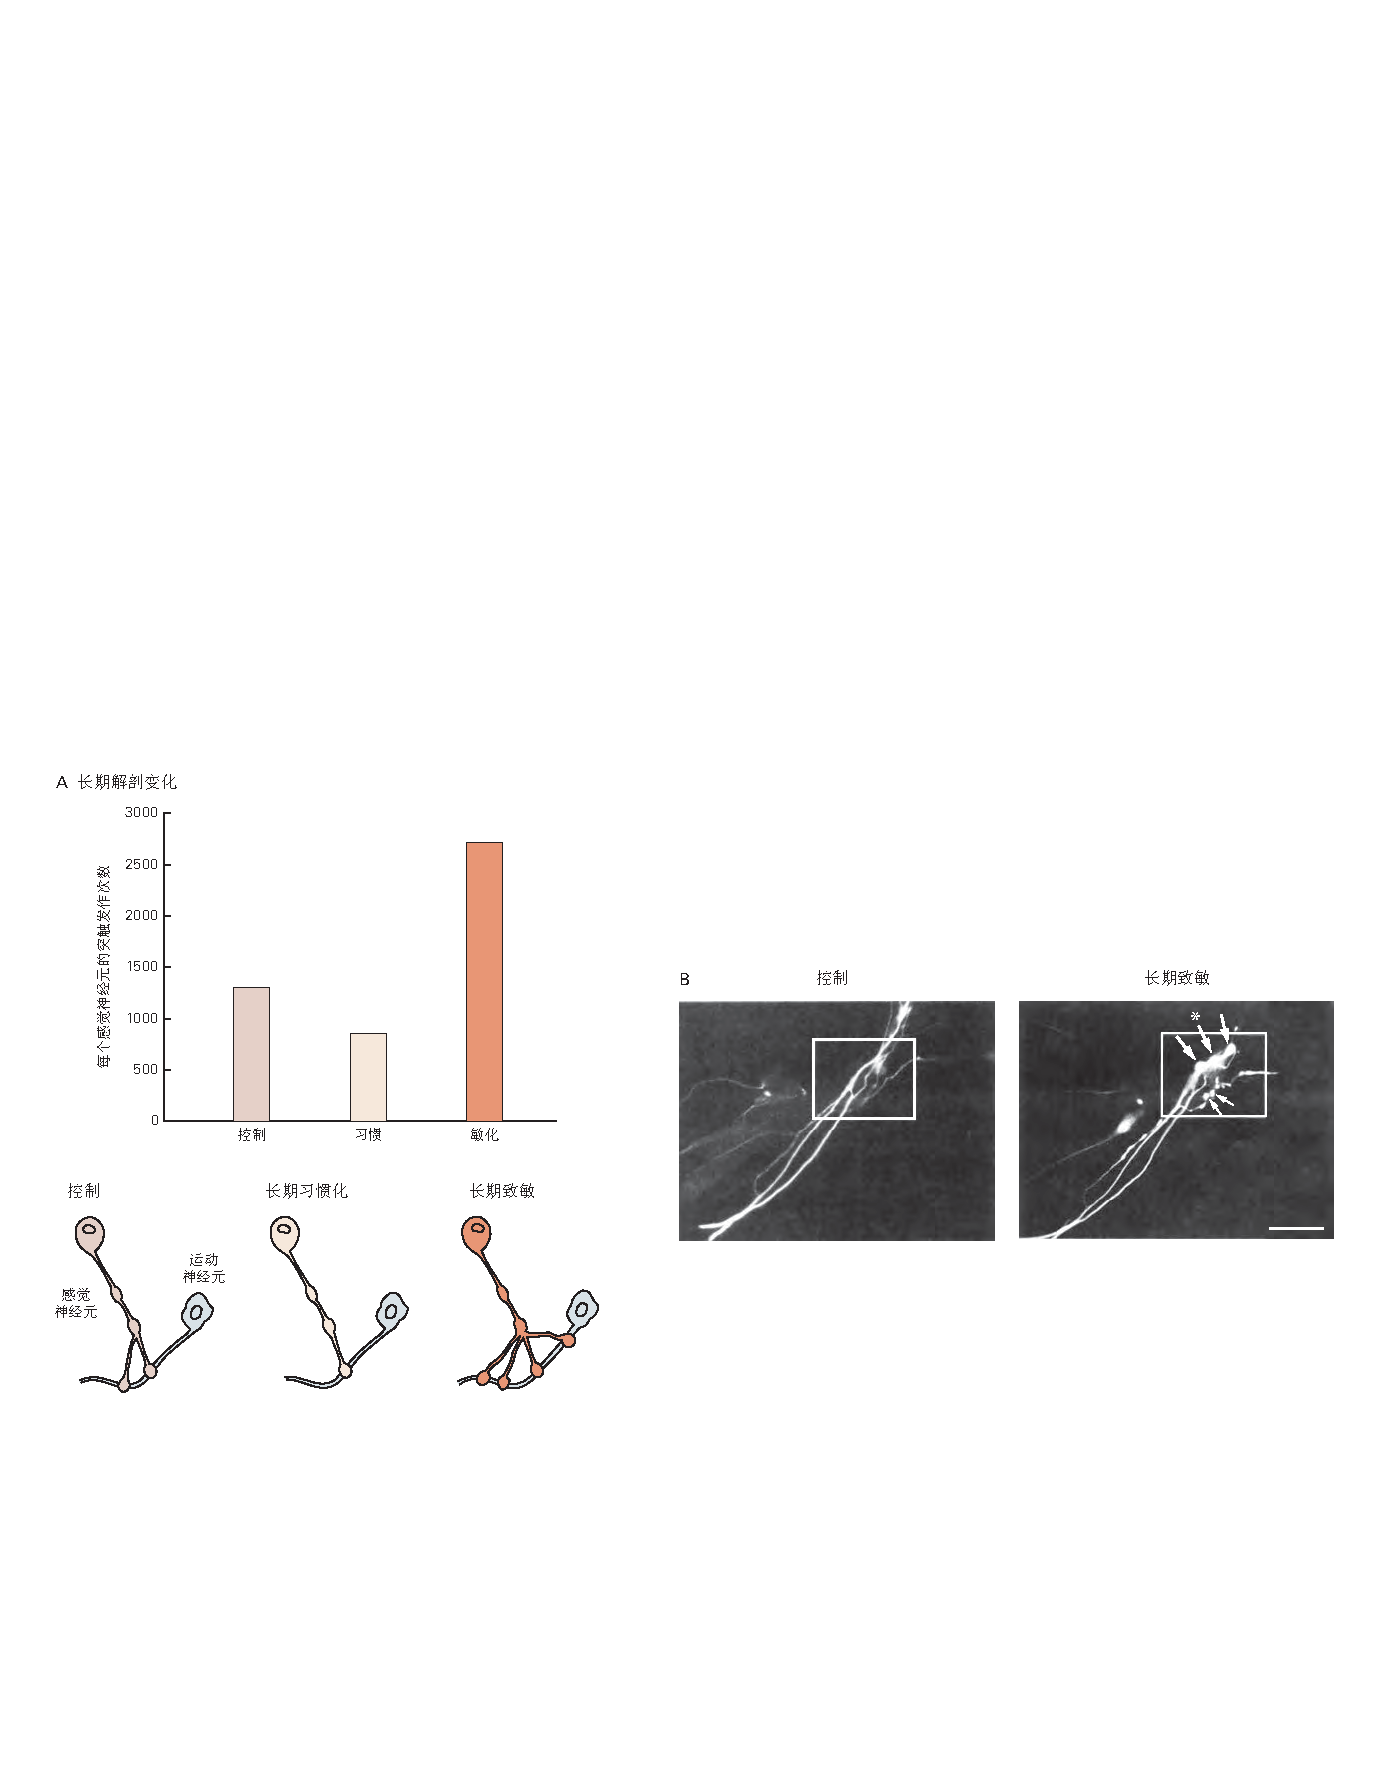
\includegraphics[width=0.95\linewidth]{chap53/fig_53_9}
	\caption{长期习惯化和敏感化涉及感觉神经元突触前末梢的结构变化。
		\textbf{A.} 长期习惯导致突触丢失,长期致敏导致突触数量增加。
		当在训练后 1 天(此处显示)或 1 周进行测量时,相对于对照水平,致敏动物的突触前末梢数量较多,而习惯动物较少。
		图表下方的图说明了突触接触数量的变化。
		感觉神经元突起上的肿胀或静脉曲张称为突触神经节;
		它们包含发射器释放所需的所有专用结构\cite{bailey1983morphological}。
		\textbf{B.} 接触培养物中的运动神经元的感觉神经元轴突在五次短暂暴露于血清素之前(左)和之后 1 天(右)的荧光图像。
		由此产生的静脉曲张增加模拟了与长期致敏相关的突触变化。
		在应用血清素之前,在轮廓区域(左)中看不到突触前静脉曲张。
		在 5-羟色胺之后,几个新的\textit{扣结}是显而易见的(箭头),其中一些包含完全发育的活性区(星号)或具有小的未成熟活性区。
		比例尺 = 50 微米\cite{glanzman1990target}。)}
	\label{fig:53_9}
\end{figure}



\subsection{长期突触促进是突触特定的}

哺乳动物大脑中一个典型的锥体神经元与范围广泛的目标细胞建立了 1 万个突触前连接。
因此,通常认为长期记忆存储应该是突触特定的——也就是说,只有那些积极参与学习的突触应该得到增强。
然而,长期促进涉及基因表达的发现——发生在细胞核中,远离神经元的突触——引发了一些关于信息存储的基本问题。


长期记忆存储确实是特定于突触的,还是在长期记忆存储过程中募集的基因产物会改变神经元中每个突触前末端的强度?
如果长期记忆是突触特异性的,那么使基因转录产物选择性地只加强某些突触而不加强其他突触的细胞机制是什么?


\textit{凯尔西·马丁}和她的同事通过使用由分离的海兔感觉神经元和分叉轴突组成的细胞培养系统解决了这些长期促进问题,该轴突与两个运动神经元形成单独的突触接触。
两个运动神经元之一的感觉神经元末梢被 5-羟色胺的局部脉冲激活,从而模拟尾部电击的神经效应。
当只施加一个血清素脉冲时,这些突触显示出短期促进作用。
第二个运动神经元上的突触没有接受血清素,突触传递没有变化。


当对同一个突触施加 5 个血清素脉冲时,这些突触显示出短期和长期促进作用,并且与运动神经元形成了新的突触连接。
虽然长期促进和突触生长需要基因转录和蛋白质合成,但未接受血清素的突触未显示突触传递增强(图~\ref{fig:53_10})。
因此,短期和长期突触促进都是突触特异性的,并且仅由那些接收调节性血清素信号的突触表现出来。


\begin{figure}[htbp]
	\centering
	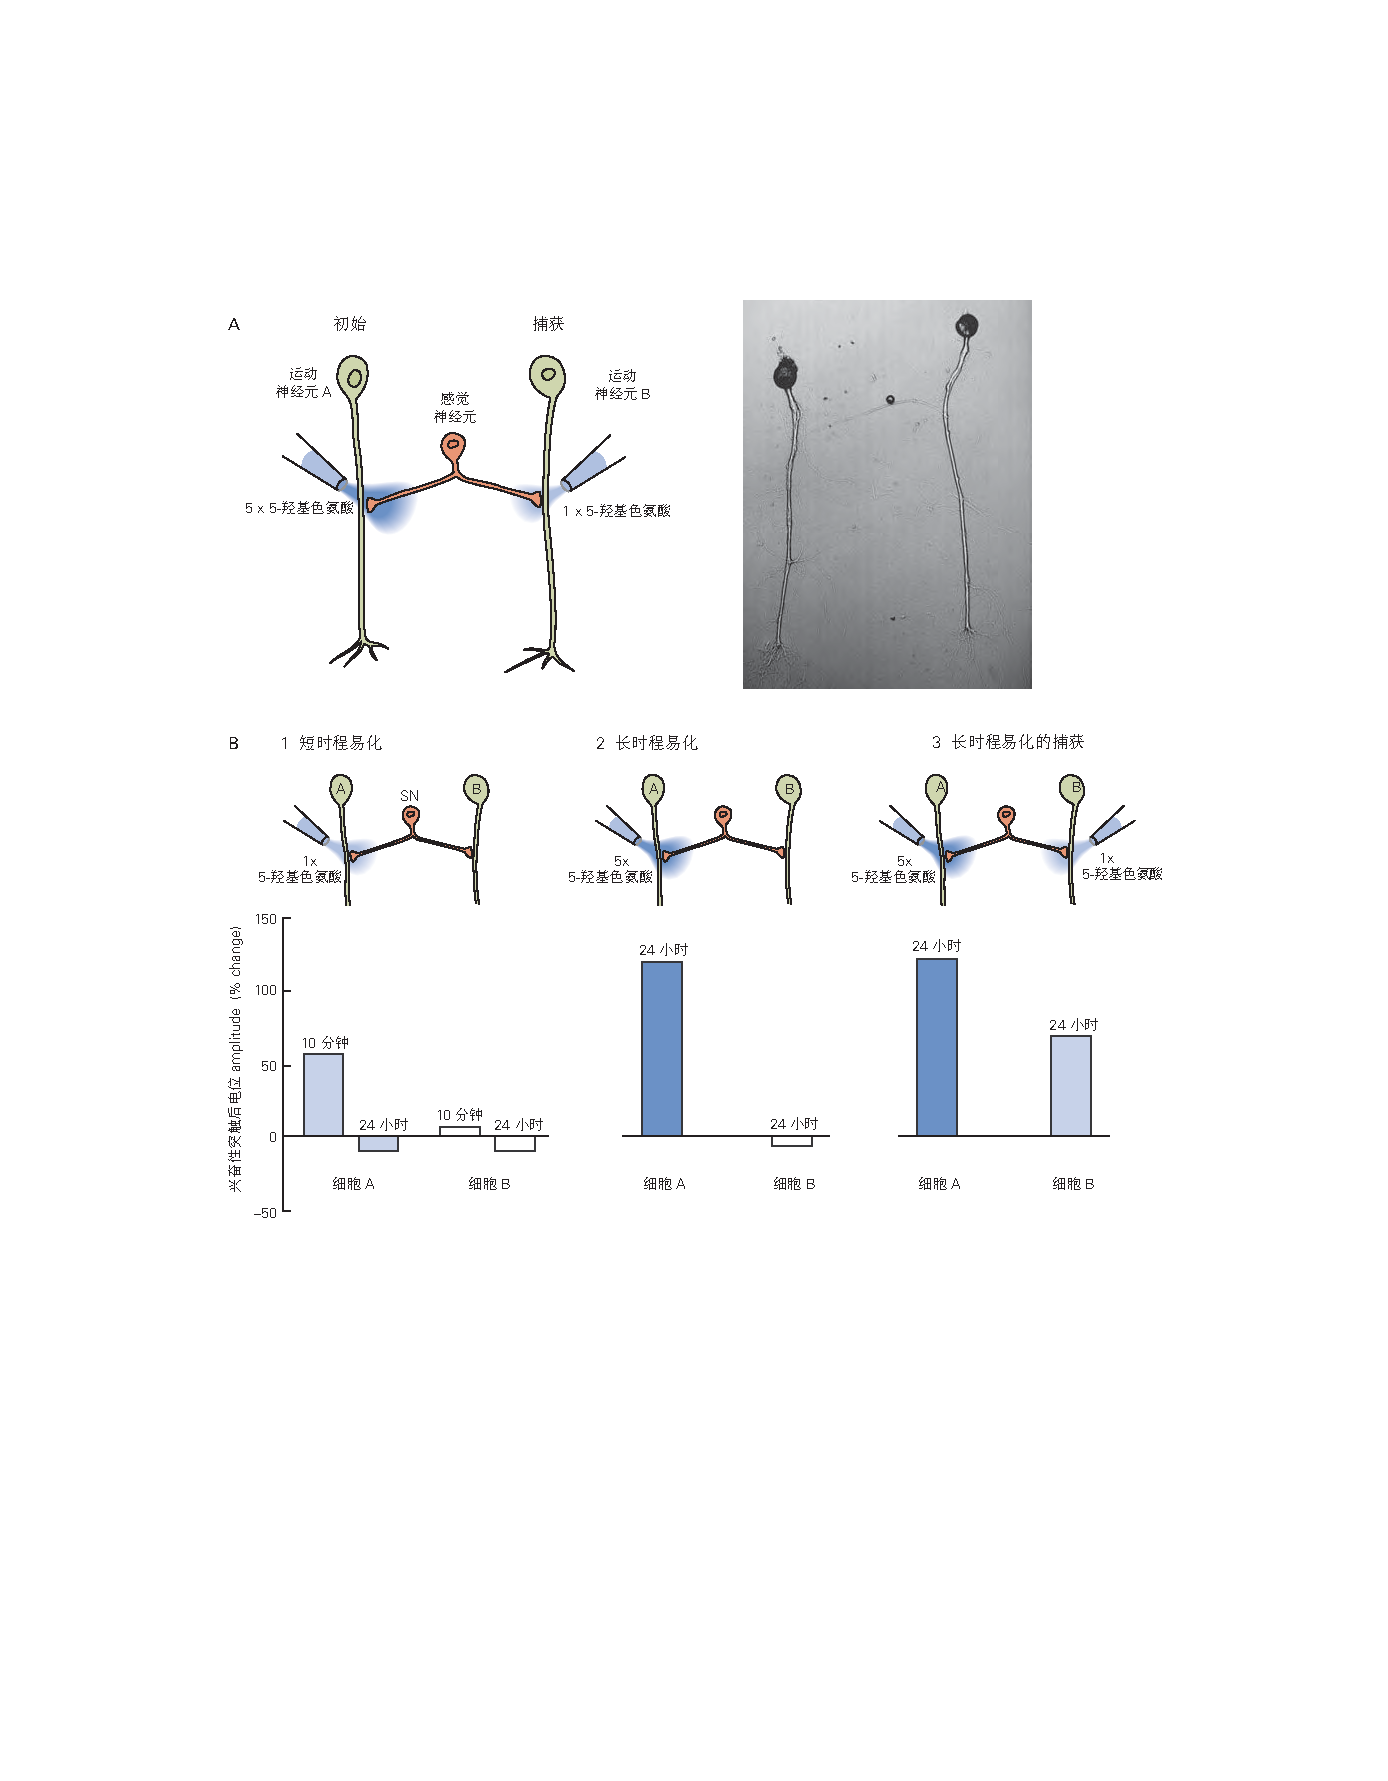
\includegraphics[width=0.95\linewidth]{chap53/fig_53_10}
	\caption{突触传递的长期促进是突触特异性的\cite{martin1997synapse}。
		\textbf{A.} 该实验使用单个突触前感觉神经元与两个突触后运动神经元 A 和 B 接触。
		左侧的吸管用于施加五个\textit{5-羟基色氨酸}脉冲与运动神经元 A 的感觉神经元突触,在该突触处启动长期促进作用。
		右侧的吸管用于将\textit{5-羟基色氨酸}的一个脉冲施加到具有运动神经元 B 的感觉神经元突触,使该突触能够利用(捕获)细胞体内产生的新蛋白质在与运动神经元 A 的突触处以响应 \textit{5-羟基色氨酸} 的五个脉冲  。
		右图显示了培养细胞的实际外观。
		\textbf{B.} 1. 将一个\textit{5-羟基色氨酸}脉冲施加到运动神经元 A 的突触上,仅对神经元中的\textit{兴奋性突触后电位}产生短期(10 分钟)促进作用。
		24 小时后,\textit{兴奋性突触后电位}已恢复到正常大小。
		细胞 B 中的\textit{兴奋性突触后电位}大小没有显着变化。
		2. 将 5 个\textit{5-羟基色氨酸}脉冲应用于细胞 A 的突触会对该细胞中的\textit{兴奋性突触后电位}产生长期(24 小时)促进作用,但大小没有变化 细胞 B 中的\textit{兴奋性突触后电位}。
		3. 当五个 5-HT 脉冲作用到细胞 A 的突触上与单个\textit{5-羟基色氨酸}脉冲作用到细胞 B 的突触上时,细胞 B 现在显示长期促进和增加 24 小时后以\textit{兴奋性突触后电位}大小。}
	\label{fig:53_10}
\end{figure}


但是,核产物如何能够仅增强某些突触的传递,而不增强同一神经元的其他突触的传递呢?
新合成的蛋白质是否以某种方式仅针对那些接受血清素的突触?
还是它们被运送到所有突触,但仅在那些至少有一个血清素脉冲标记的突触上有效地用于新突触连接的生长?


为了测试这个问题,\textit{马丁}和她的同事再次选择性地将五次血清素脉冲施加到感觉神经元与其中一个运动神经元形成的突触上。
然而,这一次,第二个运动神经元的突触同时被单次血清素脉冲激活(血清素本身只产生持续几分钟的短期突触易化作用)。
在这些条件下,5-羟色胺的单脉冲足以在感觉神经元和第二运动神经元之间的接触处诱导新突触连接的长期促进和生长。
因此,将单次血清素脉冲施加到第二个分支的突触上,使这些突触能够使用响应第一个分支突触上的五个血清素脉冲而产生的核产物,这一过程称为捕获。


这些结果表明,新合成的基因产物,包括\textit{信使核糖核酸}和蛋白质,通过快速轴突运输传递到神经元的所有突触,但仅在以先前突触活动为标志的突触处起作用,即通过血清素的突触前释放。
虽然突触上的一个血清素脉冲不足以在细胞体中开启新的基因表达,但足以标记该突触,使其能够利用细胞体中产生的新蛋白质来响应细胞体中的五个血清素脉冲 另一个突触。
这个想法由\textit{马丁}和她的同事为\textit{海兔}开发,\textit{弗雷}\textit{莫里斯}独立为啮齿动物的海马体开发,被称为突触捕获或突触标记。


这些发现提出了一个问题,允许捕获基因产物以进行长期促进的突触标记的性质是什么?
当\textit{蛋白激酶A}抑制剂局部应用于接收单次血清素脉冲的突触时,这些突触不再捕获响应五次血清素脉冲而产生的基因产物(图~\ref{fig:53_11})。
这表明\textit{蛋白激酶A}的局部磷酸化是突触捕获所必需的。


\begin{figure}[htbp]
	\centering
	\includegraphics[width=0.95\linewidth]{chap53/fig_53_11}
	\caption{长期促进需要\textit{环磷酸腺苷}依赖性磷酸化和局部蛋白质合成j\cite{casadio1999transient}。
		\textbf{A.} 5 个\textit{5-羟基色氨酸}脉冲应用于运动神经元 A 的突触,单脉冲应用于细胞 B 的突触。
		蛋白质抑制剂\textit{蛋白激酶A};Rp-cAMPS)或局部蛋白质合成(吐根碱)应用于细胞 B 上的突触。
		\textbf{B.} Rp-cAMPS 在神经元 B 的突触处完全阻断长期易化作用的捕获。
		Emetine 对捕获 促进或新突触连接的增长在\textit{5-羟基色氨酸}应用后 24 小时测量,但到 72 小时,它完全阻止突触增强。
		新突触连接的产物被缩回,如果局部蛋白质合成不维持捕获,则长期促进会在 1 天后衰减。}
	\label{fig:53_11}
\end{figure}


80 年代初期,\textit{奥斯瓦尔德·斯图尔德}发现核糖体(蛋白质合成机制)存在于突触和细胞体中。
\textit{马丁}研究了局部蛋白质合成在长期突触促进中的重要性,方法是将单次血清素脉冲与局部蛋白质合成抑制剂一起应用于一组突触,同时将五次血清素脉冲应用于第二组突触。
通常,长期促进和突触生长会持续长达 72 小时以响应突触捕获。
在存在局部蛋白质合成抑制剂的情况下,突触捕获仍然发生,在仅暴露于一次血清素脉冲的突触处产生长期突触促进。
然而,促成只持续了24小时。
24 小时后,这些突触的突触生长和易化作用崩溃,表明学习诱导的突触生长的维持需要突触处新的局部蛋白质合成(图~\ref{fig:53_11}B)。


\textit{马丁}和她的同事因此发现,突触处蛋白质合成的调节在控制海兔感觉-运动神经元连接的突触强度方面起着重要作用。
正如我们将在第~\ref{chap:chap54}~章中看到的那样,局部蛋白质合成对于海马突触强度长期增强的后期阶段也很重要。


这些发现表明海兔的突触标记有两个不同的组成部分。
第一个成分持续约 24 小时,启动长期突触可塑性和突触生长,需要在细胞核内转录和翻译,并募集局部\textit{蛋白激酶A}活性,但不需要局部蛋白质合成。
第二种成分在 72 小时后稳定长期突触变化,需要在突触处进行局部蛋白质合成。
如何调节这种局部蛋白质合成?



\subsection{维持长期突触促进需要局部蛋白质合成的类似朊病毒的蛋白质调节剂}

\textit{信使核糖核酸}在突触处翻译以响应血清素一个脉冲对该突触的标记这一事实表明,这些\textit{信使核糖核酸}最初可能处于休眠状态,并处于血清素募集的翻译调节器的控制之下。
大多数\textit{信使核糖核酸}的翻译要求转录物在其 3' 末端包含一个长尾的腺苷核苷酸 [poly(A) 尾巴]。
\textit{约尔·里希特}早些时候发现,在爪蟾(青蛙)卵母细胞中,母体\textit{信使核糖核酸}只有一条短的腺嘌呤核苷酸尾巴,因此在被\textit{胞质聚腺苷酸化元件结合蛋白}激活之前是沉默的。
\textit{胞质聚腺苷酸化元件结合蛋白}与\textit{信使核糖核酸}上的一个位点结合并募集 poly(A) 聚合酶,从而导致 poly(A) 尾部的伸长。


\textit{考斯克·斯伊}和他的同事发现,血清素增加了海兔感觉神经元末梢中一种新型神经元特异性\textit{胞质聚腺苷酸化元件结合蛋白}亚型的局部合成。
\textit{胞质聚腺苷酸化元件结合蛋白}的诱导与转录无关,但需要新的蛋白质合成。
在激活的突触处局部阻断\textit{胞质聚腺苷酸化元件结合蛋白}会阻断突触促进突触的长期维持,但不会阻断其启动和最初的 24 小时维持。


\textit{胞质聚腺苷酸化元件结合蛋白}如何稳定长期促进的后期阶段?
大多数生物分子的半衰期相对较短(几小时到几天),而记忆则持续数天、数周甚至数年。
学习引起的突触分子组成的改变如何能维持这么长时间?
大多数假设都提出了某种类型的调节突触强度和结构的自我维持机制。


Si 和他的同事惊人地发现,海兔\textit{胞质聚腺苷酸化元件结合蛋白}的神经元亚型似乎具有类似于朊病毒蛋白的自我维持特性。
朊病毒是由\textit{史坦利·布鲁希纳}发现的,他证明这些蛋白质是克雅氏病(一种毁灭性的神经退行性人类疾病)和疯牛病的病原体。
朊蛋白可以以两种形式存在:可溶形式和能够自我延续的聚集形式。
海兔\textit{胞质聚腺苷酸化元件结合蛋白}也有两种构象状态,一种是非活性的可溶形式,一种是活性的聚集形式。
该开关取决于富含谷氨酰胺的\textit{胞质聚腺苷酸化元件结合蛋白}的 N 末端结构域,类似于其他蛋白质中的朊病毒结构域。


在幼稚突触中,\textit{胞质聚腺苷酸化元件结合蛋白}以可溶、非活动状态存在,其静息表达水平较低。
然而,作为对 5-羟色胺的响应,\textit{胞质聚腺苷酸化元件结合蛋白}的局部合成增加,直到达到将\textit{胞质聚腺苷酸化元件结合蛋白}切换到聚集的活性状态的阈值浓度,然后能够激活休眠\textit{信使核糖核酸}的翻译。
一旦建立了活跃状态,它就会通过将可溶性\textit{胞质聚腺苷酸化元件结合蛋白}募集到聚集体来自我延续,从而保持其激活休眠\textit{信使核糖核酸}翻译的能力。
尽管休眠\textit{信使核糖核酸}是在细胞体中产生并分布在整个细胞中,但它们仅在具有活跃\textit{胞质聚腺苷酸化元件结合蛋白}聚集体的突触处被翻译。


虽然传统的朊病毒机制是致病的——大多数朊病毒蛋白的聚集状态会导致细胞死亡——海兔\textit{胞质聚腺苷酸化元件结合蛋白}是一种新型的朊病毒样蛋白,其聚集状态起着重要的生理功能。
海兔\textit{胞质聚腺苷酸化元件结合蛋白}的主动自我延续形式在突触中维持长期的分子变化,这是记忆存储持久性所必需的(图 \ref{fig:53_12})。


\begin{figure}[htbp]
	\centering
	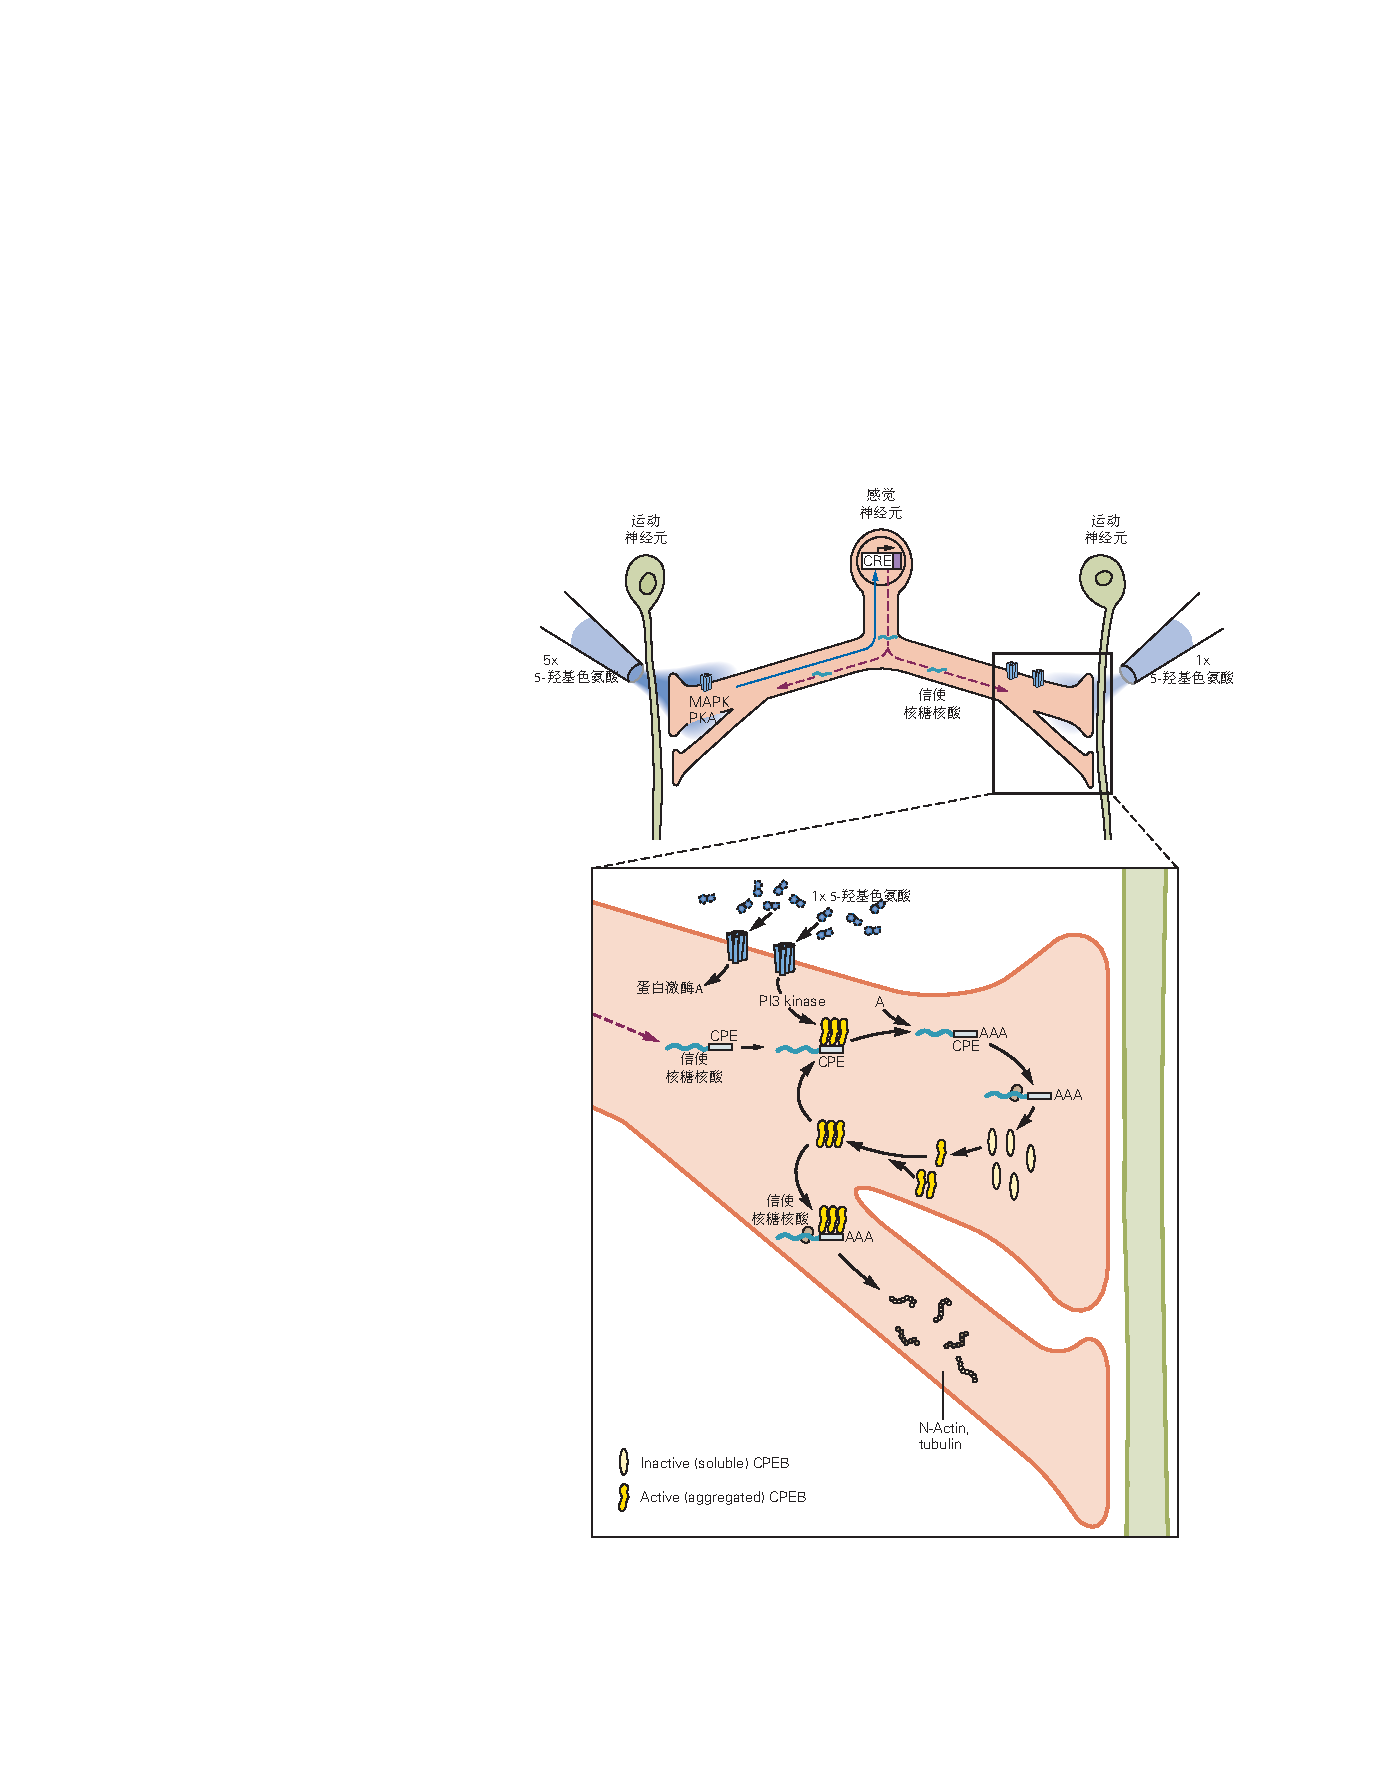
\includegraphics[width=0.75\linewidth]{chap53/fig_53_12}
	\caption{海兔轴突末端蛋白质合成的自我延续开关可维持长期突触促进。
		五个\textit{5-羟基色氨酸}脉冲会产生一个信号,该信号会返回细胞核以激活\textit{信使核糖核酸}的合成。
		然后通过快速轴突运输将细胞体中新转录的\textit{信使核糖核酸}和新合成的蛋白质发送到所有终端。
		然而,只有那些被至少一个血清素脉冲标记的终端才能使用这些蛋白质来生长长期促进所需的新突触。
		终端的标记涉及两种物质:
		(1) \textit{蛋白激酶A},它是运输到终端的蛋白质启动的即时突触生长所必需的,以及 (2) 磷酸肌醇 3 激酶(PI3 激酶),它启动维持突触生长和超过 24 小时的长期促进所需的\textit{信使核糖核酸}的局部翻译。 末端的一些\textit{信使核糖核酸}编码\textit{胞质聚腺苷酸化元件结合蛋白},这是一种局部蛋白质合成的调节剂。
		在基础状态下,\textit{胞质聚腺苷酸化元件结合蛋白}被认为以一种基本无活性的构象存在,作为一种不能与\textit{信使核糖核酸}结合的可溶性单体。
		通过血清素和 PI3 激酶激活的一些尚未明确的机制,\textit{胞质聚腺苷酸化元件结合蛋白}的一些拷贝转化为形成聚集体的活性构象。
		聚集体的功能类似于朊病毒,因为它们能够招募单体加入聚集体,从而激活单体。
		\textit{胞质聚腺苷酸化元件结合蛋白}聚集体结合\textit{信使核糖核酸}的细胞质聚腺苷酸化元件 (CPE) 位点。
		这种结合会招募 poly(A) 聚合酶机制,并允许将腺嘌呤核苷酸 (A) 的 poly(A) 尾巴添加到休眠的\textit{信使核糖核酸}中。
		多聚腺苷酸化的\textit{信使核糖核酸}现在可以被核糖体识别,从而允许将这些\textit{信使核糖核酸}翻译成几种蛋白质。
		例如,除了\textit{胞质聚腺苷酸化元件结合蛋白}之外,这还会导致 N-肌动蛋白和微管蛋白的局部合成,从而稳定新生长的突触结构\cite{bailey2004persistence}。}
	\label{fig:53_12}
\end{figure}


\subsection{存储在感觉运动突触中的记忆在检索后变得不稳定但可以重新稳定}

\textit{卡里姆·奈德}和其他人对哺乳动物进行的多项研究发现,在其早期阶段,长期记忆存储是动态的,可能会被打乱。
特别是,记忆痕迹在检索后可能变得不稳定,需要额外一轮巩固(所谓的再巩固)。


直到最近,尚不清楚参与存储记忆的同一组突触是否在检索后不稳定和重新稳定,或者在记忆后突触重新激活后,一组新的突触是否受到调节。
对这个问题进行了检查,以恢复海兔鳃和虹吸管\textit{缩鳃反射}的长期敏感性。
这些实验表明,由于泛素介导的蛋白质降解,恢复的记忆变得不稳定,然后通过新蛋白质合成的方式重新巩固。


在经过长期促进的感觉运动突触中是否会发生类似的再巩固机制?
事实上,当经过长期促进的突触被突触前动作电位的短暂爆发重新激活时,该突触会因蛋白质降解而变得不稳定,需要蛋白质合成才能重新稳定。
这些结果表明,记忆的再巩固涉及在存储初始记忆的相同突触处重新稳定突触促进。



\section{果蝇防御反应的经典威胁条件反射也使用 \textit{环磷酸腺苷}-\textit{蛋白激酶A}-\textit{环磷酸腺苷应答元件结合蛋白} 途径}

在海兔中发现的内隐记忆存储的细胞机制是否与其他动物相似?
对厌恶学习的研究表明,同样的机制也被用于果蝇果蝇和啮齿动物的记忆存储,表明后生动物进化过程中的保守机制。
果蝇对于内隐记忆存储的研究特别方便,因为它的基因组很容易被操纵,而且正如\textit{西摩·本泽}和他的同事首先证明的那样,果蝇可以进行经典调节。
在典型的经典条件反射范例中,气味伴随着对脚的反复电击。
然后通过允许苍蝇在迷宫的两条臂之间进行选择来检查学习的程度,其中一条臂包含与电击配对的气味,另一条臂包含未配对的气味。
训练后,大部分野生型苍蝇会避开带有条件气味的手臂。
已经确定了几种不会学会避免条件气味的果蝇突变体。
这些学习有缺陷的突变体被赋予了富有想象力的描述性名称,例如 dumb、dunce、\textit{芜菁甘蓝
}、\textit{健忘症}和 \textit{蛋白激酶A}-R1。
非常有趣的是,所有这些突变体都在\textit{环磷酸腺苷}级联中存在缺陷。


嗅觉调节取决于苍蝇大脑中称为蘑菇体的区域。
蘑菇体的神经元,称为\textit{凯尼恩细胞},接收来自触角叶的嗅觉输入,触角叶的结构类似于哺乳动物大脑的嗅叶。
\textit{凯尼恩细胞}细胞还接收来自多巴胺能神经元的输入,这些神经元对厌恶刺激(例如足部电击)有反应。
多巴胺与促代谢受体(由 dumb 基因编码)结合,后者激活刺激性 G 蛋白和特定类型的 \ce{Ca^2+}/钙调蛋白依赖性腺苷酸环化酶(由芜菁甘蓝基因编码),类似于参与海兔经典条件反射的环化酶。
由无条件刺激(足部电击)释放的多巴胺的收敛作用和由嗅觉输入触发的细胞内 \ce{Ca^2+} 的升高导致腺苷酸环化酶的协同激活,从而产生\textit{环磷酸腺苷}的大量增加。


最近的实验表明,当气味剂与多巴胺能神经元的直接刺激配对时,苍蝇可以进行经典调节,绕过足部电击。
在这些实验中,哺乳动物 P2X 受体(\textit{三磷酸腺苷}门控阳离子通道)在多巴胺能神经元中表达为转基因。
然后给果蝇注射笼中的\textit{三磷酸腺苷}衍生物。
多巴胺能神经元然后可以通过将光照在果蝇上以从其笼中释放\textit{三磷酸腺苷}并激活 P2X 受体来激发动作电位。
当多巴胺能神经元在气味存在的情况下以这种方式被激活时,果蝇就会进行厌恶调节——它们学会避开气味。
因此,无条件刺激会激活多巴胺信号,从而加强厌恶条件反射,就像血清素在海兔中充当习得防御反应的厌恶强化信号一样。


反向遗传学方法也被用于探索果蝇的记忆形成。
在这些实验中,各种转基因置于热敏启动子的控制之下。
热敏感性允许基因通过升高容纳苍蝇的腔室的温度来随意打开。
这是在成熟动物身上进行的,以尽量减少对大脑发育的任何潜在影响。
当\textit{蛋白激酶A}的催化亚基被抑制性转基因的瞬时表达阻断时,果蝇无法形成短期记忆,表明\textit{环磷酸腺苷}信号转导通路对于果蝇的联想学习和短期记忆的重要性。


果蝇的长期记忆需要新的蛋白质合成,就像海兔和其他动物一样。
\textit{环磷酸腺苷应答元件结合蛋白}激活基因的敲除有选择地阻断长期记忆而不干扰短期记忆。
相反,当基因过度表达时,通常只产生短期记忆的训练过程会产生长期记忆。


与海兔一样,果蝇中某些形式的长期记忆也涉及\textit{胞质聚腺苷酸化元件结合蛋白},并且可能依赖于这种蛋白质中的朊病毒样行为。
雄性果蝇在接触不接受的雌性后学会抑制它们的求爱行为。
当\textit{胞质聚腺苷酸化元件结合蛋白}的 N 末端结构域被基因删除时,长期求爱记忆就会丧失;
雄性苍蝇无法识别不接受的雌性。
该 N 末端结构域富含谷氨酰胺残基,对应于海兔\textit{胞质聚腺苷酸化元件结合蛋白}中富含谷氨酰胺的朊病毒样结构域。
因此,涉及内隐记忆的几种分子机制从海兔到苍蝇都是保守的,正如我们接下来将看到的,这种保守延伸到哺乳动物。



\section{哺乳动物的威胁学习记忆涉及杏仁核}

过去几十年的研究已经详细了解了哺乳动物对威胁的先天和后天防御反应的神经回路,通常称为“恐惧学习”。
特别是,正如我们在第~\ref{chap:chap42}~章中提到的,这两种类型的防御反应都与杏仁核有关,杏仁核参与检测和评估范围广泛的重要且具有潜在危险的环境刺激。
基于杏仁核的防御系统可以快速了解新的危险。
它可以在单次配对暴露后将新的中性刺激(条件刺激)与已知威胁(非条件刺激)联系起来,并且这种习得的关联通常会终生保留。


杏仁核直接从感觉系统接收有关威胁的信息。
杏仁核的输入核,即外侧核,是来自无条件和条件刺激的信号的汇聚点。
这两种信号都由一条从丘脑直接到达杏仁核的快速通路和一条从丘脑投射到新皮层的感觉区并从那里到达杏仁核的较慢的间接通路传送。
这些平行通路都有助于调节(图 \ref{fig:53_13})。
杏仁核还通过来自皮层联合区的连接接收高阶认知信息,尤其是额叶和颞叶的内侧皮质区域。


\begin{figure}[htbp]
	\centering
	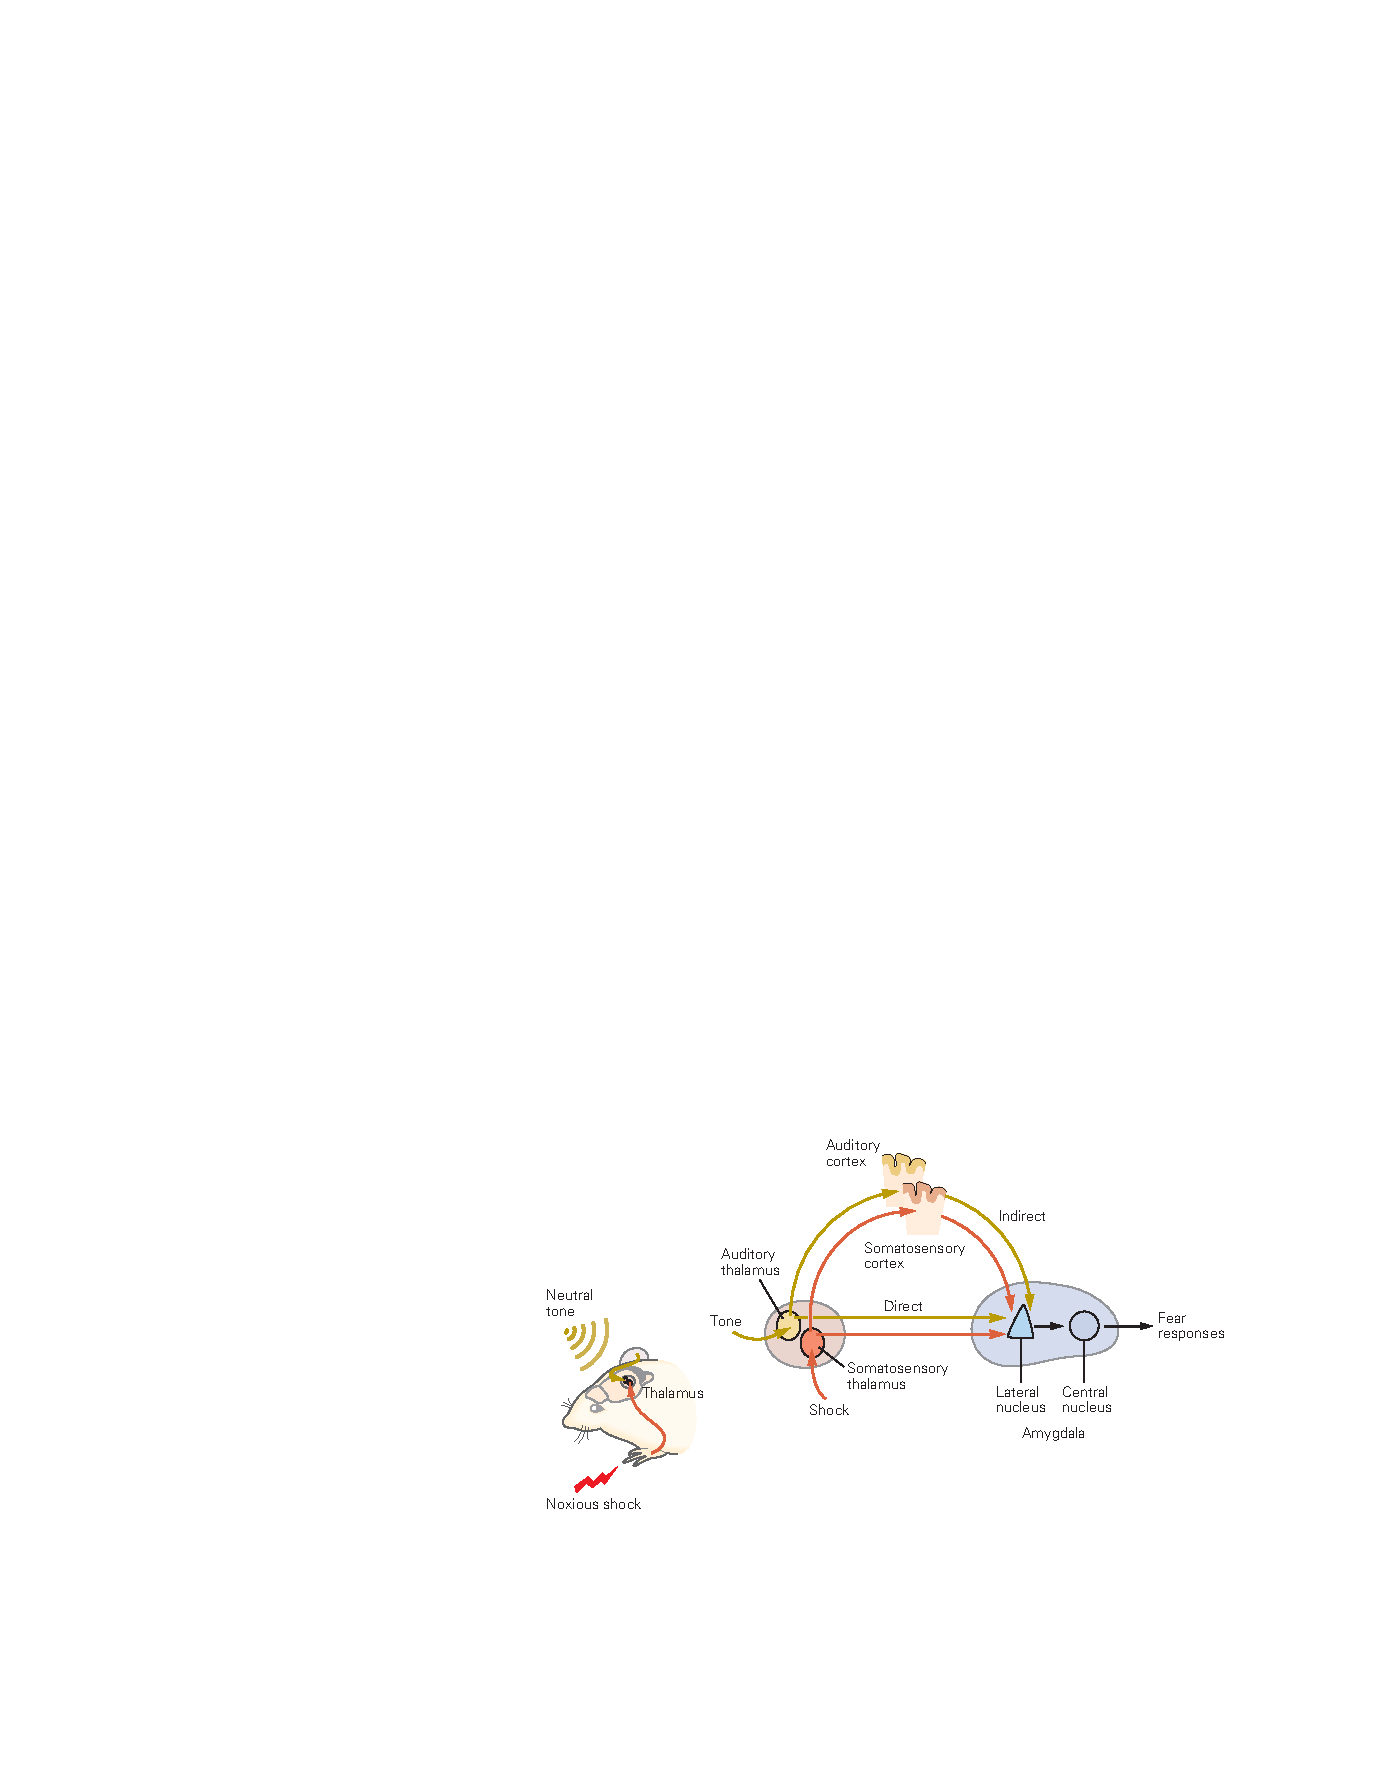
\includegraphics[width=0.75\linewidth]{chap53/fig_53_13}
	\caption{威胁学习涉及从\textit{丘脑}到\textit{杏仁核}的平行通路。
		条件刺激的信号(此处为中性音调)通过两条途径从\textit{听觉丘脑}传递到杏仁核\textit{外侧核}:通过\textit{直接}途径和通过听觉皮层的\textit{间接}途径。
		类似地,无条件刺激的信号(这里是电击)通过平行的伤害感受通路从丘脑的体感部分传递到外侧核,一个是直接通路,一个是通过体感皮层的间接通路。
		外侧核依次投射到中央核,即杏仁核的输出核,它激活神经回路,增加心率,产生其他自主神经变化,并引发构成防御状态的防御行为\cite{kandel2007search}。}
	\label{fig:53_13}
\end{figure}


在巴甫洛夫条件反射期间,杏仁核中的突触传递强度发生了变化。
响应于音调,与兴奋性突触反应成比例的细胞外电生理信号被记录在侧核中。
在将音调与电击配对后,突触传递的增加会增强对音调的电生理反应,这取决于音调(条件刺激)和电击(非条件刺激)在外侧杏仁核中的单个神经元上的收敛(图~\ref{fig:53_14})。


\begin{figure}[htbp]
	\centering
	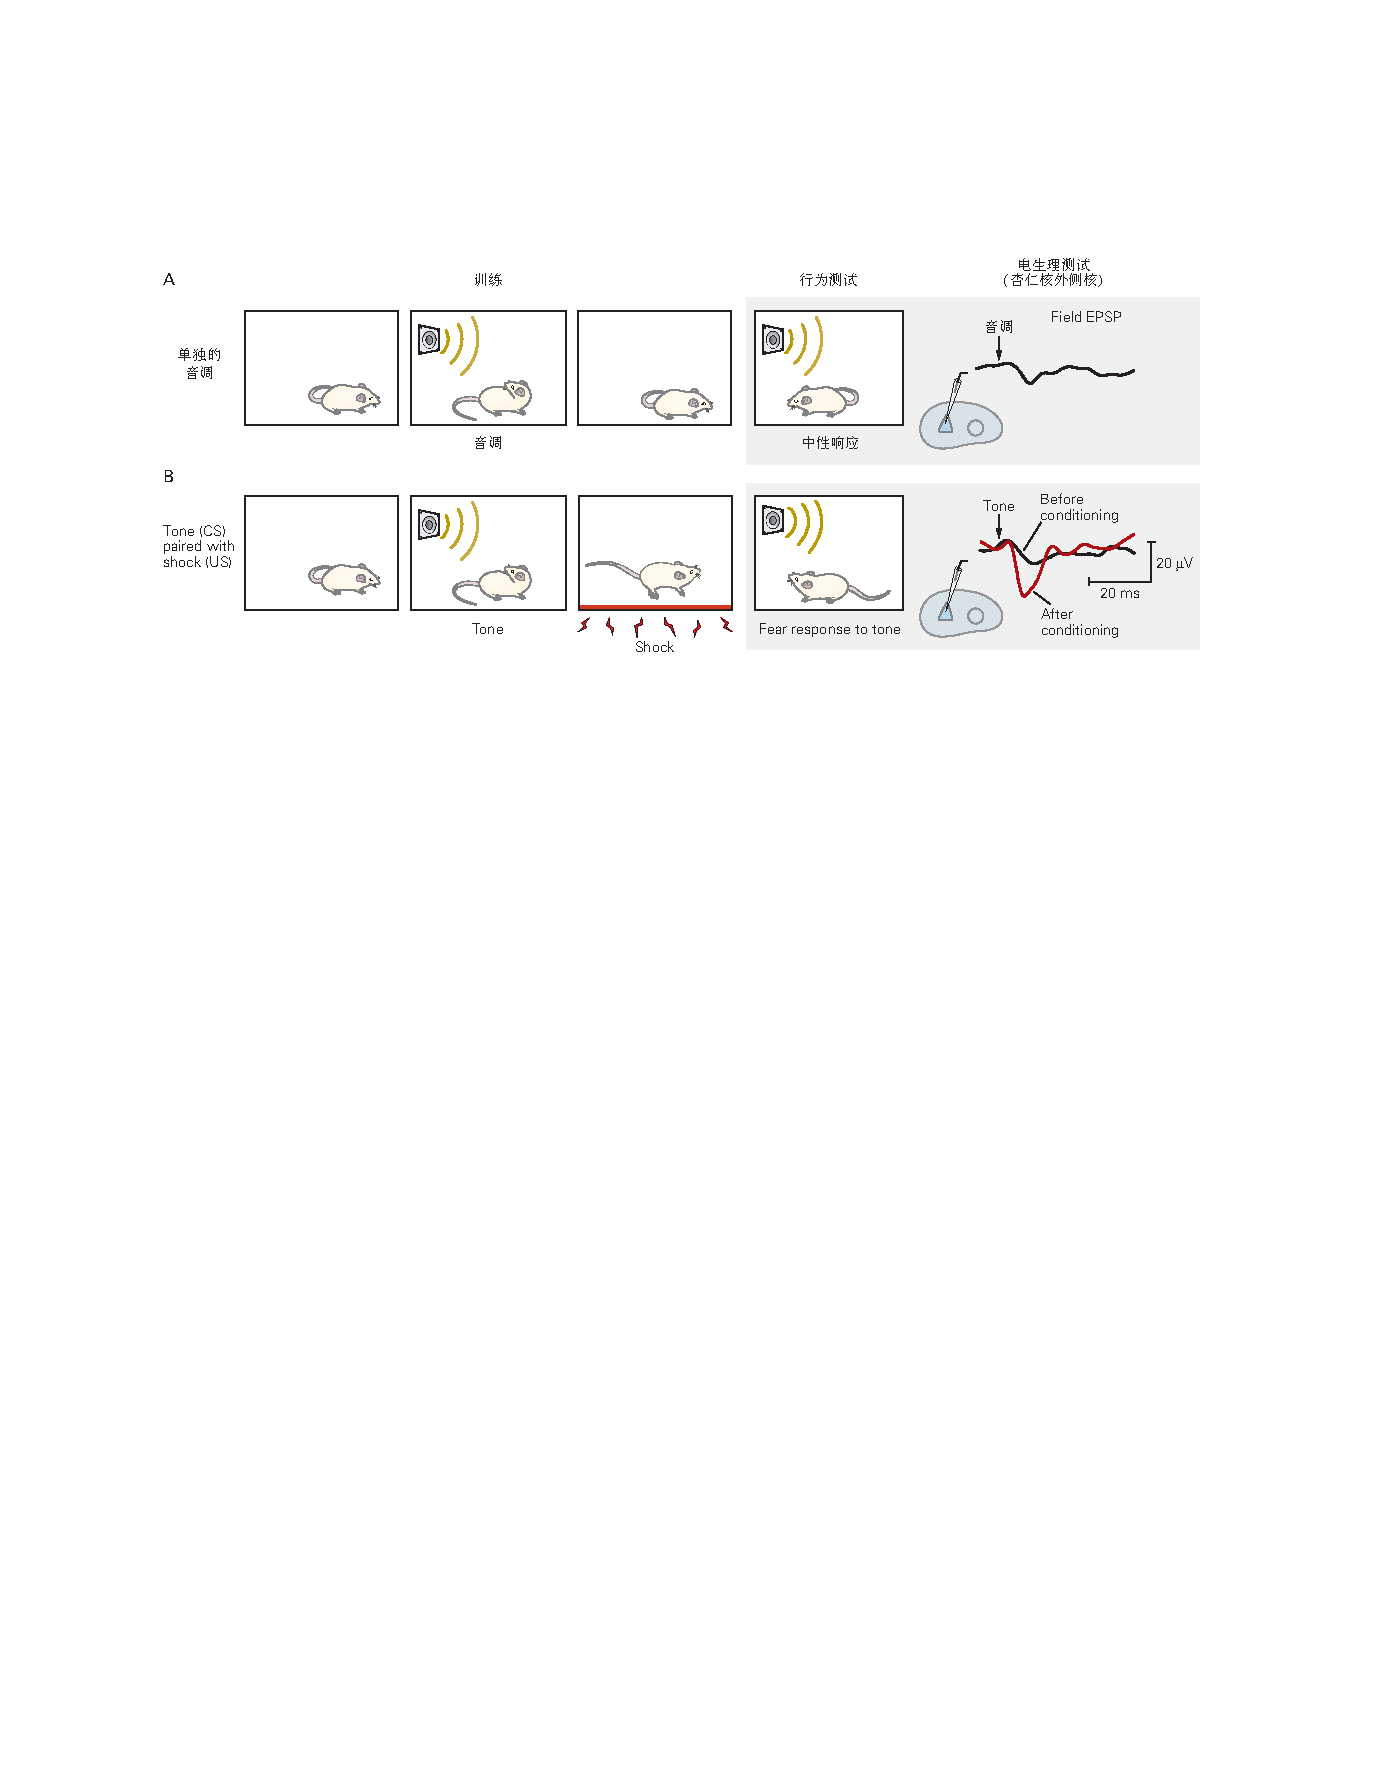
\includegraphics[width=1.0\linewidth]{chap53/fig_53_14}
	\caption{威胁学习会产生相关的行为和电生理变化。
		\textbf{A.} 动物通常会忽略中性音调。
		音调在细胞外场电极记录的\textit{杏仁核}中产生小的突触反应。 
		当兴奋性突触电流进入大量杏仁核神经元的树突时,杏仁核中的记录电极与大脑外部的第二电极之间的小电压降会产生场\textit{兴奋性突触后电位}。
		\textbf{B.} 当音调在足部电击前立即出现时,动物学会将音调与电击联系起来。
		结果,单是音调就会引起先前引起的震惊:它会导致鼠标冻结,这是一种本能的防御反应。
		威胁条件反射后,杏仁核外侧核对音调的电生理反应大于条件反射前的反应\cite{rogan2005distinct}。}
	\label{fig:53_14}
\end{figure}


人们普遍认为行为学习取决于突触可塑性。
为了了解在外侧杏仁核的学习过程中这种可塑性是如何发生的,研究人员研究了\textit{长时程增强},这是一种可塑性细胞模型。
我们最初在第~\ref{chap:chap13}~章讨论了与兴奋性突触功能相关的\textit{长时程增强},并将在第~\ref{chap:chap54}~章结合外显记忆和海马体对其进行详细研究。
在包括外侧杏仁核的脑切片中,\textit{长时程增强}可以通过直接或间接感觉通路的高频强直刺激来诱导,这会导致对这些输入的兴奋性突触后反应的持久增加。
这种变化是由一种形式的同突触可塑性引起的(图~\ref{fig:53_15})。


\begin{figure}[htbp]
	\centering
	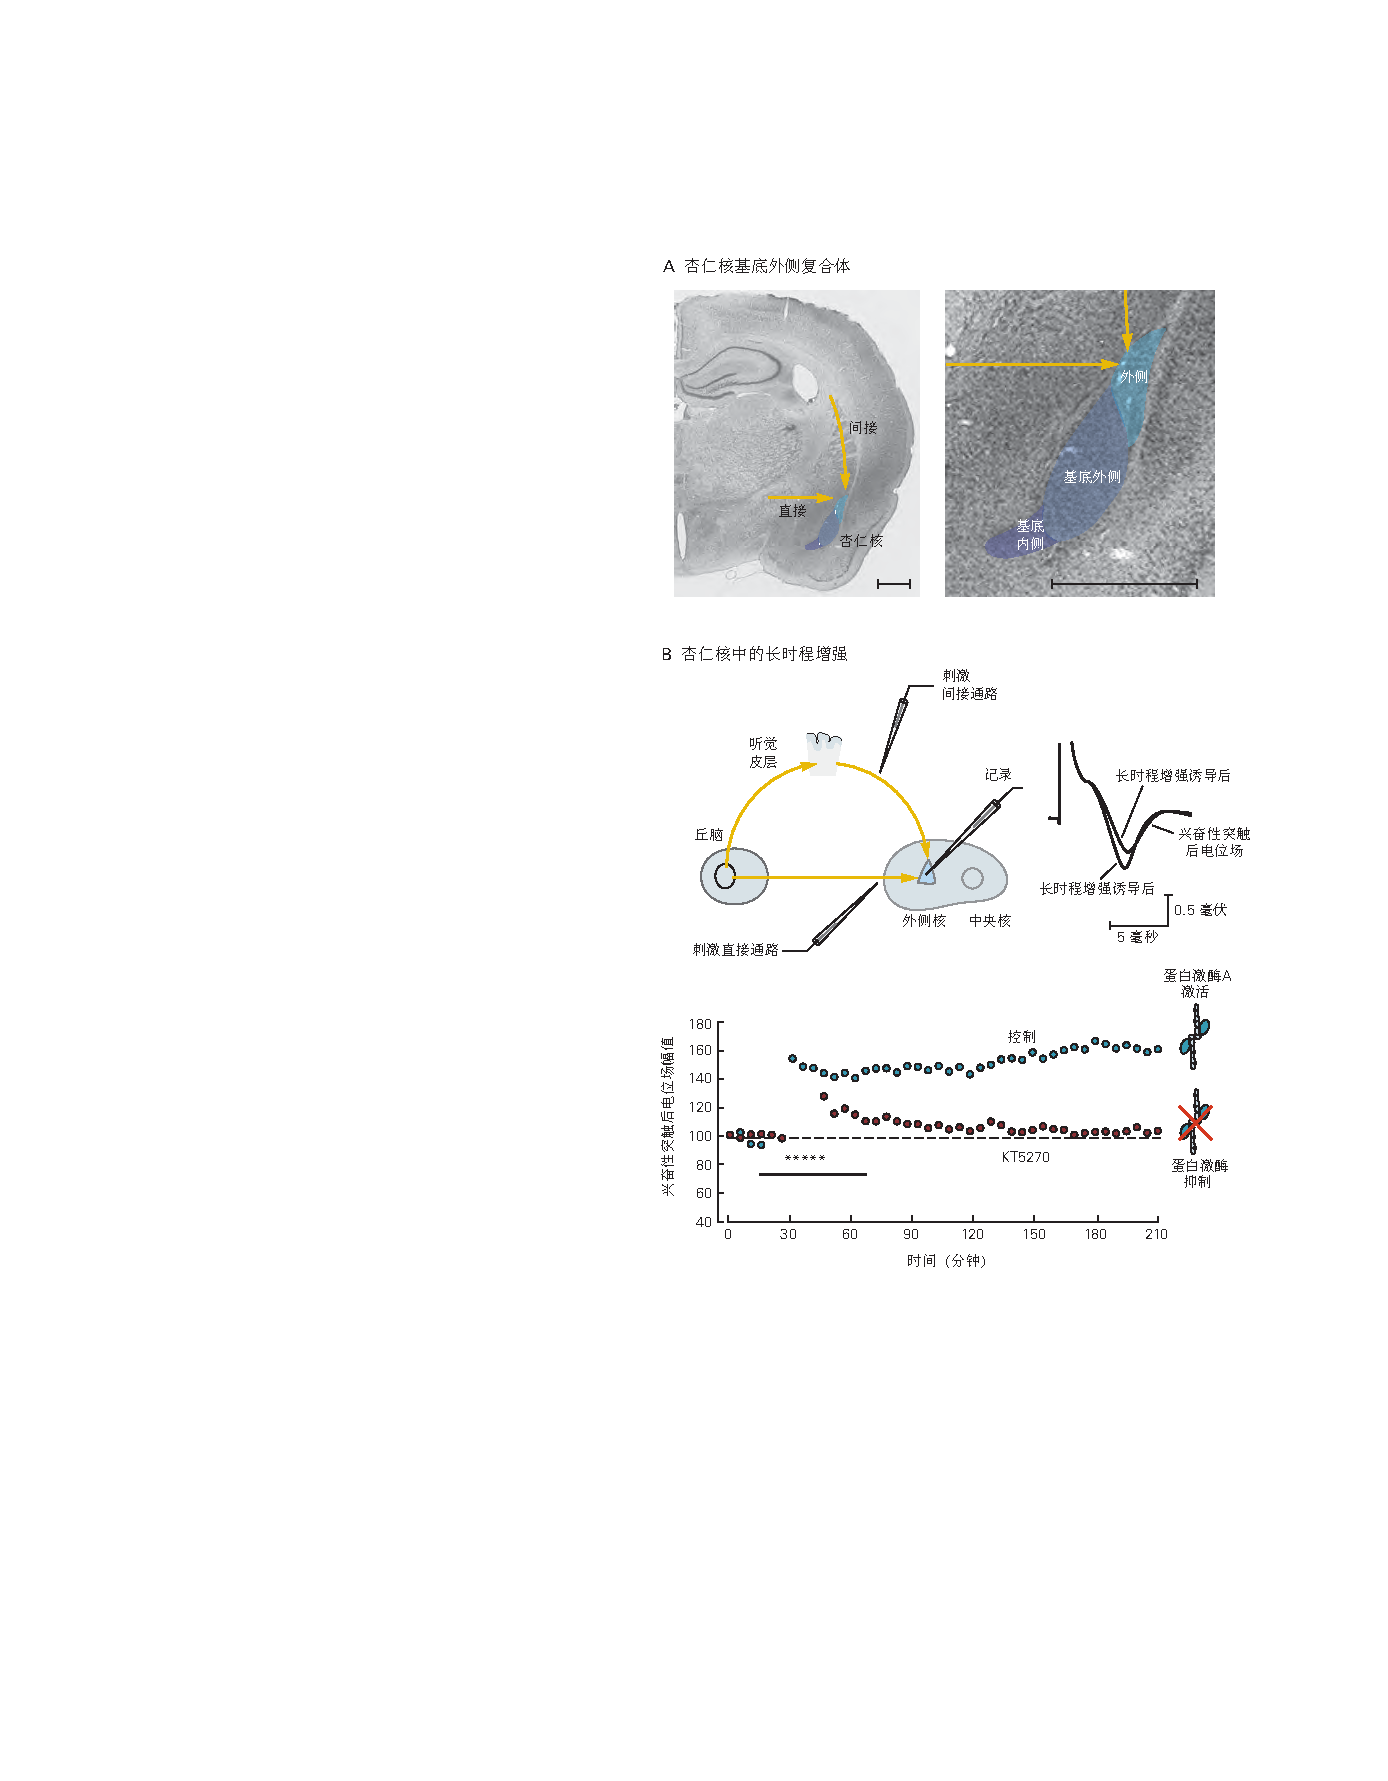
\includegraphics[width=0.7\linewidth]{chap53/fig_53_15}
	\caption{杏仁核中突触的长期增强可能会介导威胁条件反射。
		\textbf{A.} 小鼠的冠状脑切片显示了杏仁核的位置。
		放大图显示了杏仁核的三个关键输入核——\textit{外侧}、\textit{基底外侧}和\textit{基底内侧}——它们一起形成了基底外侧复合体。
		这些核投射到中央核,中央核投射到下丘脑和脑干\cite{maren1999long}。
		\textbf{B.} 从丘脑到侧核的直接或间接通路的高频强直刺激启动\textit{长时程增强}。
		该图显示了细胞外电压记录电极在侧核中的位置,以及用于激活直接通路或间接通路的两个刺激电极的位置。
		该图显示了在实验过程中细胞外场\textit{兴奋性突触后电位}响应间接皮层通路刺激的振幅。
		当以低频率(每 30 秒一次)刺激通路时,场\textit{兴奋性突触后电位}是稳定的。
		然而,当应用五列高频强直刺激(星号)时,反应会增强数小时。
		这种促进作用取决于\textit{蛋白激酶A},并且在应用 \textit{蛋白激酶A} 抑制剂 KT5720 时会受到影响(柱状图)。 还显示了诱导\textit{长时程增强}之前和之后的现场\textit{兴奋性突触后电位}\cite{huang1998postsynaptic,huang2000both}。}
	\label{fig:53_15}
\end{figure}


杏仁核外侧核的长时程增强是由 \ce{Ca^2+} 流入突触后神经元以响应强烈的突触活动而触发的。
\ce{Ca^2+} 进入是由突触后细胞中\textit{N-甲基-D-天冬氨酸}型谷氨酸受体和 L 型电压门控 \ce{Ca^2+} 通道的打开介导的。
因为\textit{N-甲基-D-天冬氨酸}受体通常被细胞外 \ce{Mg^2+} 阻断,所以它们需要大量的突触输入来产生足够的突触后去极化以解除这种阻滞(第 \ref{chap:chap13} 章)。
L 型通道也需要强烈的去极化才能打开。 因此,\textit{长时程增强}仅在响应同时发生的突触活动时产生。
钙流入会触发生化级联反应,通过在突触后膜中插入额外的\textit{α-氨基-3-羟基-5-甲基异恶唑-4-丙酸}型谷氨酸受体和增加神经递质释放来增强突触传递 突触前终端。
与海兔一样,在强直性刺激期间释放的单胺类神经递质,如去甲肾上腺素和多巴胺,提供有助于诱导 \textit{长时程增强}的异突触调节信号。


对清醒行为的啮齿动物的研究表明,类似的机制有助于获得巴甫洛夫威胁条件反射。
这种学习形式需要外侧杏仁核中的突触后\textit{N-甲基-D-天冬氨酸}受体和电压门控钙通道,并且它会被外侧杏仁核中蓝斑释放的去甲肾上腺素增强。


此外,在先前受过训练的动物的杏仁核切片中通过电刺激引发的\textit{长时程增强}的大小小于未经训练的动物切片中发现的\textit{长时程增强}。
因为可以增强突触的数量存在上限,所以这一结果被视为威胁条件反射招募\textit{长时程增强}的证据,这阻止了进一步的\textit{长时程增强}响应电刺激。
因此,人工诱导的\textit{长时程增强}和行为诱导的\textit{长时程增强}密切相关。


两种类型的基因实验也有力地支持了\textit{长时程增强}样现象有助于细胞机制存储习得威胁记忆的观点。
首先,\textit{N-甲基-D-天冬氨酸}受体的 GluN2B (NR2B) 亚基的遗传破坏会干扰威胁条件反射和\textit{长时程增强}在将条件刺激信号传输到外侧杏仁核的通路中的诱导。
此外,这种突变只影响习得的威胁;
它不影响对无条件威胁或常规突触传递的反应。
相反,GluN2B 亚基的过度表达有助于学习。 同样,\textit{环磷酸腺苷应答元件结合蛋白}信号的中断(\ce{Ca^2+} 流入的下游步骤)会干扰条件反射,而\textit{环磷酸腺苷应答元件结合蛋白}活动的增强会促进学习。


如在脑切片中观察到的那样,对威胁学习重要的\textit{长时程增强}是否涉及插入新的\textit{α-氨基-3-羟基-5-甲基异恶唑-4-丙酸}受体?
为了解决这个问题,研究人员用一种基因工程病毒感染了侧核中的锥体神经元,这种病毒不会损害神经元,但会导致它们表达带有荧光标记的\textit{α-氨基-3-羟基-5-甲基异恶唑-4-丙酸}受体。
威胁调节导致标记的\textit{α-氨基-3-羟基-5-甲基异恶唑-4-丙酸}受体插入细胞膜的增加,类似于在脑切片中实验诱导的\textit{长时程增强}期间所见。
当使用另一种病毒来表达\textit{α-氨基-3-羟基-5-甲基异恶唑-4-丙酸}受体的 C 末端部分,该部分与内源性\textit{α-氨基-3-羟基-5-甲基异恶唑-4-丙酸}受体竞争并阻止其插入时,对习得威胁的记忆大大减少,即使该病毒仅感染了 10\% 到 20\% 的\textit{α-氨基-3-羟基-5-甲基异恶唑-4-丙酸}受体。
侧核中的神经元。 这一令人惊讶的结果表明,几乎所有激活的突触都需要诱导\textit{长时程增强}才能有效支持威胁学习。


巴甫洛夫范式的优点之一是它易于进行实验研究,因为特定刺激通过已知途径传递到杏仁核。
这使得实验者能够直接激活条件刺激或非条件刺激通路,绕过正常的感官输入。
这些研究提供了令人信服的证据,表明这些通路与威胁学习中的杏仁核有关。


基于这些发现,研究人员探讨了当他们将听觉条件刺激(音调)与外侧杏仁核神经元的直接去极化配对时是否可以诱导威胁学习,而不是使用外部的、引起疼痛的无条件冲击刺激来通过无条件的去极化产生去极化。
外侧杏仁核的刺激通路。 为此,他们使用了光遗传学方法(第~\ref{chap:chap5}~章)。
他们将一种病毒注入杏仁核,以在外侧杏仁核神经元中表达视紫红质通道蛋白 2,这是一种光激活的兴奋性阳离子通道。
在将听觉刺激与使外侧杏仁核细胞去极化的光脉冲配对后,仅音调的呈现会引起条件性冻结。
当存在去甲肾上腺素时,冻结量更大,这进一步证明调节通路也在该回路的突触促进中发挥作用。
因此,厌恶冲击本身并不是诱导威胁学习所必需的。
相反,关键是刺激与外侧杏仁核激活的关联。


其他研究证明了人为操纵杏仁核以损害和实例化威胁记忆的可能性。
他们首先训练动物将足部电击与杏仁核听觉输入的光遗传学刺激联系起来。
然后,他们传递了一种光遗传学刺激模式,使杏仁核的听觉输入产生\textit{长时程抑制},这是一种突触可塑性形式,其中微弱的重复刺激会降低突触传递的强度。
\textit{长时程抑制}的感应能够使休克的记忆失活。
然后,使用产生相同听觉输入的\textit{长时程增强}的光刺激模式,他们发现可以恢复对电击的记忆。
可以使用\textit{长时程抑制}和\textit{长时程增强}设计记忆的失活和重新激活的发现加强了突触强度和行为记忆存储之间可能的因果关系。


威胁记忆背后的突触变化的持久性取决于杏仁核中的基因表达和蛋白质合成,很像海兔和果蝇的长期记忆。
因此,\textit{环磷酸腺苷}依赖性蛋白激酶和 \textit{有丝分裂原活化蛋白激酶} 激活转录因子\textit{环磷酸腺苷应答元件结合蛋白}以启动基因表达。
\textit{环磷酸腺苷应答元件结合蛋白}的重要性通过发现外侧杏仁核中的不同神经元在威胁条件反射之前具有不同水平的\textit{环磷酸腺苷应答元件结合蛋白}表达而得到强调。
在学习过程中选择性地招募表达高于平均\textit{环磷酸腺苷应答元件结合蛋白}量的神经元。
相反,如果\textit{环磷酸腺苷应答元件结合蛋白}静息水平高的神经元在学习后被选择性消融,记忆就会受损。


虽然关于威胁条件反射的神经机制的大部分工作都涉及杏仁核的外侧核,但近年来,越来越多的证据表明中央核的可塑性也很重要。
中央核接收来自侧核的直接和间接输入,并与中脑导水管周围灰色区域的神经元形成突触连接,投射到脑干以控制许多防御反应,包括冻结行为。
在中央核的外侧细胞群中,称为\textit{蛋白激酶C}$ \delta $ 神经元的抑制性细胞控制投射到导水管周围灰质的内侧细胞群中的输出神经元的活动。


人类的威胁条件反射记忆也涉及杏仁核。
因此,在人类中,杏仁核的损伤会损害威胁条件反射的内隐记忆,但不会损害已经受到条件反射的外显记忆。
功能成像研究发现,杏仁核会被威胁激活,即使人们没有意识到威胁的存在,因为刺激是潜意识的。
尽管人类研究在揭示神经生物学细节方面的能力有限,但它们证明了动物研究与人类精神病理学的相关性。


总之,巴甫洛夫威胁条件反射已成为研究哺乳动物大脑中联想学习和记忆的最有用的实验模型之一。
部分原因是行为范式已成功应用于从苍蝇到人类的不同物种,因此建立在无脊椎动物模型取得的早期进展之上。



\section{学习引起的大脑结构变化有助于个性的生物学基础}

长期记忆存储所需的突触解剖学改变在多大程度上改变了成熟大脑的大规模功能结构?
初级躯体感觉皮层的身体表面图在不同个体之间的差异反映了他们对特定感觉通路的使用,这一事实很好地说明了答案。
这一非凡的发现是根据个人的特定经验,大脑皮层中感觉通路的连接会扩张或收缩(第~\ref{chap:chap49}~章)。


作为行为结果的传入输入的重组在大脑的较低水平也很明显,特别是在背柱核水平,其中包含躯体感觉系统的第一个突触。
因此,组织变化可能发生在整个躯体传入通路中。


经验改变皮层中体感输入图的过程在一项实验中得到了说明,在该实验中,成年猴子被训练为使用中间三个手指而不是其他手指来获取食物。
在对这种行为进行数千次试验后,中指的皮层区域大大扩大(图~\ref{fig:53_16}A)。
因此,实践可以通过加强现有连接的有效性来扩展突触连接。


\begin{figure}[htbp]
	\centering
	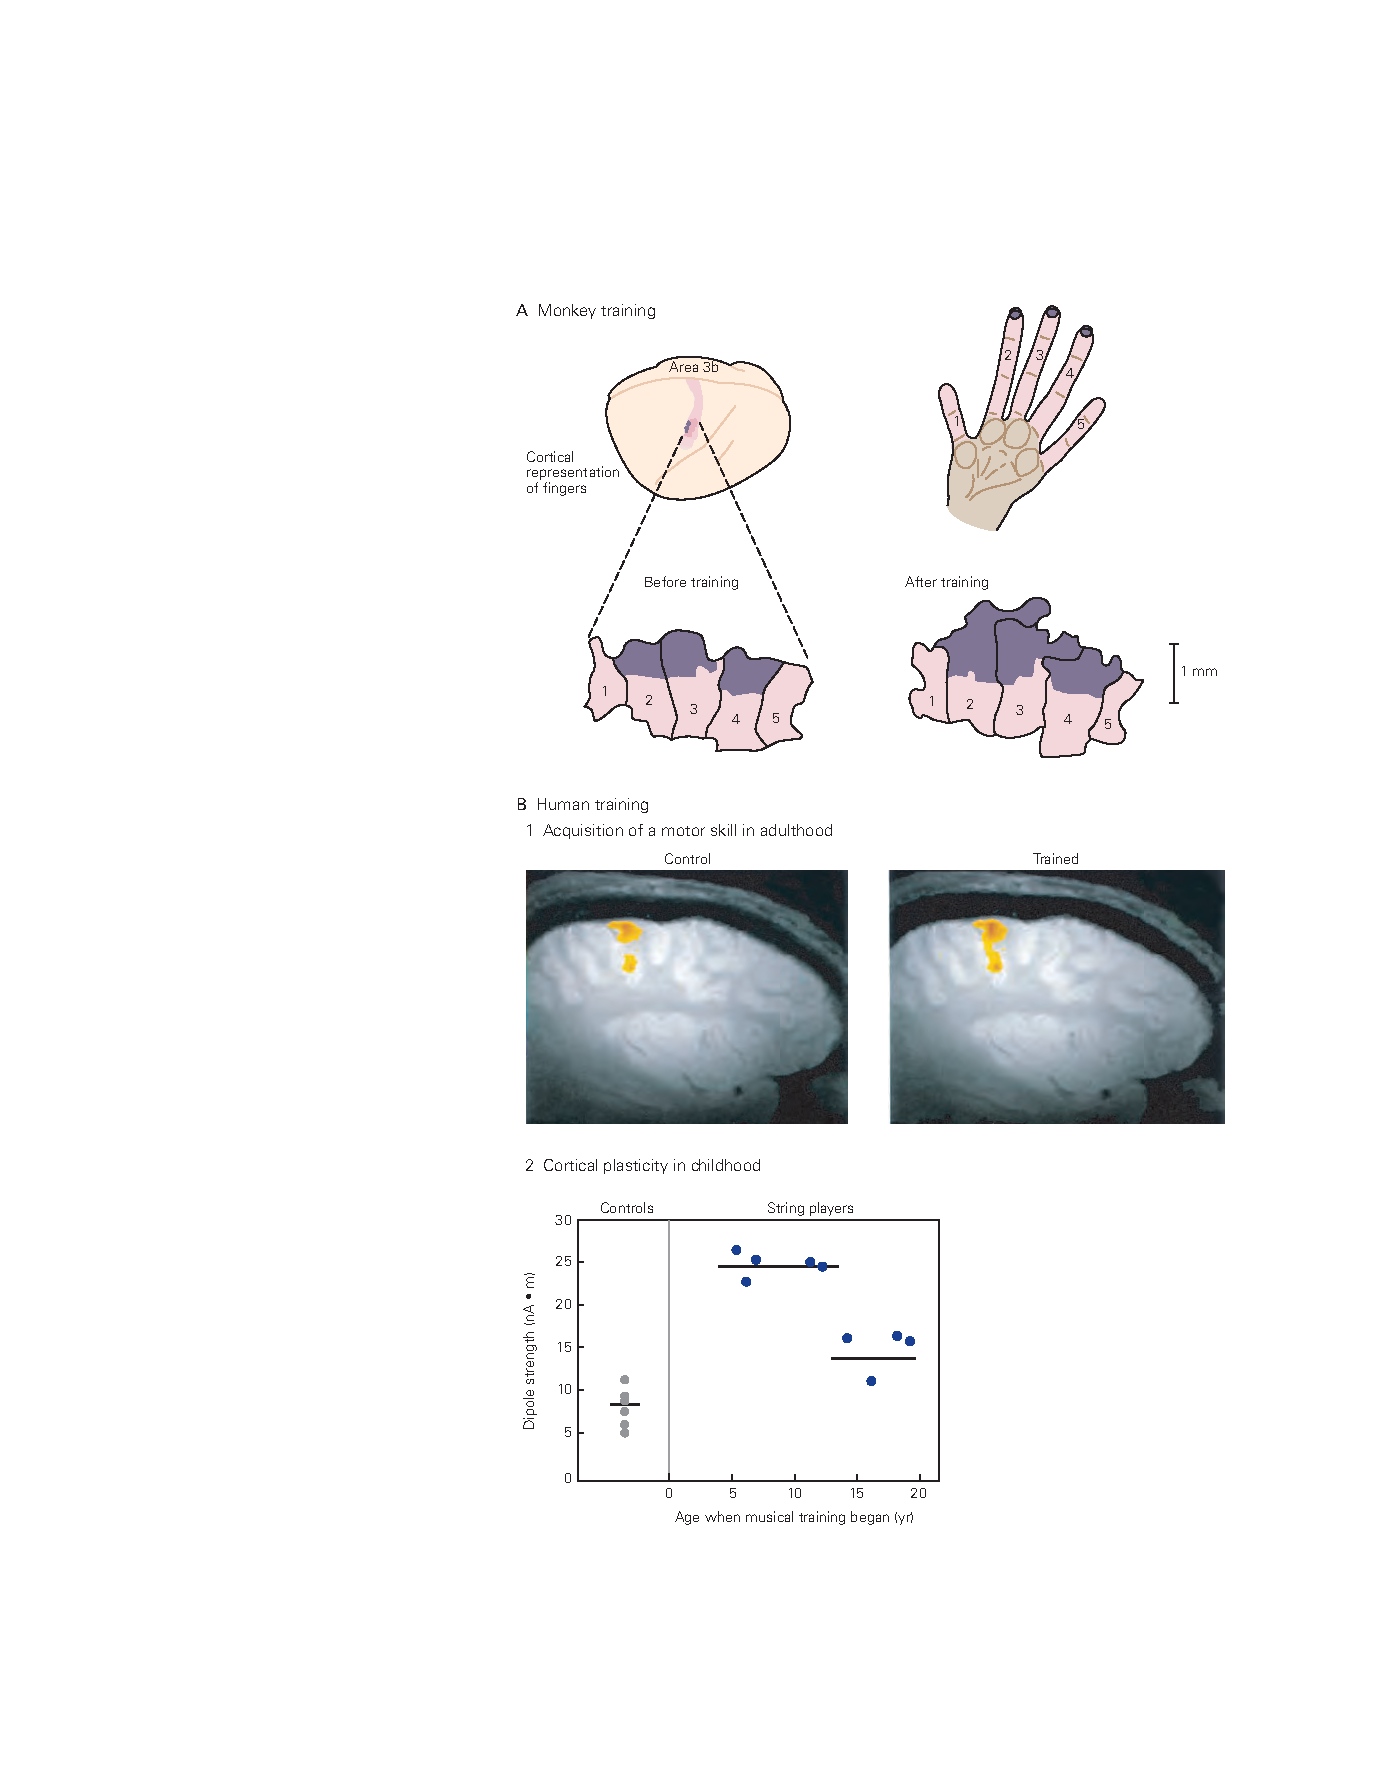
\includegraphics[width=1.0\linewidth]{chap53/fig_53_16}
	\caption{训练扩展了大脑皮层中手指输入的表示。
		\textbf{A.} 一只猴子每天接受 1 小时的训练,以执行一项需要重复使用指尖 2、3 和偶尔使用 4 的任务。
		训练后,体感皮层区域 3b 的部分代表受刺激的指尖 手指(深色)明显大于正常值(训练前 3 个月测量)\cite{jenkins1990functional}。
		\textbf{B.} 1. 经过 3 周的日常训练(每天 10-20 分钟),受过快速手指运动序列训练的人类受试者将提高准确性和速度。
		训练后初级运动皮层的功能性磁共振成像扫描(基于局部血氧水平依赖信号)显示,受过训练的受试者(橙色区域)激活的区域大于未受过训练(对照)的激活区域。
		对照组受试者未接受任何训练,并使用与对照组受试者相同的手进行未学习的手指运动。
		受过训练的受试者皮层表征的变化持续了几个月。
		2. 弦乐演奏者的左手小指皮层代表的大小比非音乐家大。
		该图绘制了从脑磁图获得的偶极子强度,脑磁图是神经活动的一种测量方法。
		这种增长在 13 岁之前开始接受音乐训练的音乐家中最为明显\cite{elbert1995increased}。}
	\label{fig:53_16}
\end{figure}


皮层神经元的体感输入的正常发育可能取决于相邻传入轴突的活动水平。
在一项使用猴子的实验中,两个相邻手指的皮肤表面通过手术连接在一起,这样连接的手指总是一起使用,从而确保它们的传入体感轴突正常被激活。
结果,体感皮层中接收来自这些数字的输入的区域之间通常明显的不连续性被消除了。
因此,皮层中相邻手指表征边界的正常发育不仅可以通过遗传来引导,还可以通过经验来引导。
皮层连接的微调可能取决于\textit{长时程增强}等联想机制,类似于合作活动在塑造视觉系统中眼优势柱发展中的作用(第~\ref{chap:chap49}~章)。


这种可塑性在人类身上也很明显。
受过训练用手指执行任务的人在执行任务期间显示初级运动皮层中的\textit{功能性磁共振成像}信号扩展(图~\ref{fig:53_16}B)。
\textit{托马斯·艾尔伯特}探索了弦乐器演奏者运动皮层中的手部表征。
这些音乐家用左手弹奏琴弦,以高度个性化的方式操纵手指。
相比之下,用于鞠躬的右手几乎像握拳一样使用。
右手在弦乐器演奏者皮层中的表征与非音乐家的相同。
但左手的代表性比非音乐家更大,并且在 13 岁之前开始演奏乐器的玩家中更为突出(图~\ref{fig:53_16}B)。


因为我们每个人都在不同的环境中长大,经历不同的刺激组合并以不同的方式发展运动技能,所以每个人的大脑都经过独特的改造。
这种大脑结构的独特改变,连同独特的基因构成,构成了个性的生物学基础。



\section{亮点}

1. 人格的许多方面都受内隐记忆的引导。
我们所经历的很多事情——我们所感知的、所想的、幻想的——并不是直接由有意识的思想控制的。


2. 在哺乳动物中,先天和习得的防御反应都涉及杏仁核。
基于杏仁核的防御系统可以快速了解新的危险。
它可以将新的中性(有条件的)刺激与已知的威胁性(无条件的)刺激联系起来,进行一次配对接触,并且这种习得的关联通常会终生保留。


3. 在巴甫洛夫条件反射期间,通过配对条件刺激和非条件刺激,外侧杏仁核中的突触传递强度被改变。
结果,外侧杏仁核中神经元的电生理反应得到增强,行为学习发生。


4. 无脊椎动物威胁条件反射的许多分子机制也有助于哺乳动物的条件反射。


5. 对人类杏仁核的损害会损害内隐威胁条件反射,但不会影响已被条件反射的外显记忆。


6. 习惯是通过重复逐渐养成的惯例,是一种独特形式的内隐学习的结果。
与所有形式的内隐学习一样,习惯仅在行动中表现出来,没有意识控制,并且独立于口头报告。


7. 正如这些论点所表明的那样,无意识心理过程的实证研究多年来因缺乏合适的实验方法而受到严重限制。
然而,今天,生物学拥有范围广泛的经验方法,这些方法提供了细胞和分子的见解,从而扩大了我们对范围广泛的心理活动的理解。


